\documentclass[12pt, letterpaper]{report}

% --- Paquetes ---
\usepackage[utf8]{inputenc}
\usepackage[spanish, es-tabla]{babel}
\usepackage[margin=2.5cm]{geometry}
\usepackage{graphicx}
\usepackage{booktabs}
\usepackage{array}
\usepackage{subcaption}
\usepackage{amsmath}
\usepackage{amssymb}
\usepackage{float}
\usepackage[table,svgnames]{xcolor}
\usepackage{xltabular}
\usepackage{cite}
\usepackage{hyperref}

% Preámbulo necesario:

 \usepackage{siunitx}

% Secciones 1, 2, 3... (report numera como capítulo.sección; este documento no usa \chapter)
\counterwithout{section}{chapter}
\counterwithout{figure}{chapter}
\counterwithout{table}{chapter}
\counterwithout{equation}{chapter}

\newcolumntype{L}{>{\raggedright\arraybackslash}X}

% --- Título ---
\title{
    
\includegraphics[width=10cm]{logofacultad1.png}\\
    Proyecto 4: 2do Avance \\ Dron 6"}

\author{Lucas Garcia \\ Hernan Ibarra}
\date{2026 - Segundo ciclo}

\begin{document}

\maketitle

% 1. Resumen Ejecutivo
\renewcommand{\abstractname}{Resumen Ejecutivo}
\begin{abstract}
    \noindent El presente proyecto tiene como objetivo el diseño y desarrollo de un controlador de vuelo (flight controller, FC) para vehículos aéreos no tripulados (UAV) de ala rotatoria tipo multirrotor, con énfasis en la versatilidad funcional y la compatibilidad con ecosistemas de hardware comercial ampliamente adoptados en la industria.
El sistema se centra en un microcontrolador STM32F405RGT6 de STMicroelectronics, basado en arquitectura ARM Cortex-M4 con unidad de punto flotante (FPU) a 168 MHz, el cual provee el rendimiento computacional necesario para ejecutar algoritmos de estimación de actitud y control de vuelo en tiempo real. La plataforma de firmware objetivo es Betaflight, estándar de facto en aplicaciones de vuelo de alto rendimiento.
En cuanto a la instrumentación embebida, el FC integra una unidad de medición inercial (IMU), que combina giroscopio y acelerómetro de seis ejes con ruido ultrabajo, un sensor barométrico para estimación de altitud mediante medición de presión absoluta y un magnetómetro para definir un compás. Adicionalmente, el diseño contempla la incorporación de un módulo GPS con interfaz UART, orientado a funciones de navegación asistida y recuperación autónoma ante pérdida de señal de control.
La arquitectura de comunicaciones incluye receptores de radiocontrol mediante protocolo ELRS (ExpressLRS) de largo alcance, telemetría bidireccional hacia estación en tierra, y salidas de control de motores mediante protocolo DSHOT sobre cuatro canales. El diseño incorpora además almacenamiento de datos de vuelo mediante interfaz SDIO hacia tarjeta microSD, interfaz USB para configuración en tierra, y soporte para transmisor de video FPV analógico.
El factor de forma adoptado es de 40×40 mm con agujeros de montaje M3 a separación estándar de 30x30 mm, asegurando compatibilidad directa con ESC 4-en-1 y demás módulos del stack comercial de drones de 5 pulgadas. El PCB se implementa en seis capas con control de impedancia diferencial para USB y single-ended para SDIO, garantizando integridad de señal en las interfaces de alta frecuencia del sistema.
\end{abstract}

% 2. Abstract
\renewcommand{\abstractname}{Abstract}
\begin{abstract}
    \noindent This project aims to design and develop a flight controller (FC) for rotary-wing unmanned aerial vehicles (UAV) of the multirotor type, with emphasis on functional versatility and compatibility with commercially adopted hardware ecosystems. The system is centered around an STM32F405RGT6 microcontroller from STMicroelectronics, based on an ARM Cortex-M4 architecture with floating-point unit (FPU) at 168 MHz, which provides the computational performance required to execute attitude estimation algorithms and flight control in real time. The target firmware platform is Betaflight, the de facto standard in high-performance flight applications.
Regarding embedded instrumentation, the FC integrates an inertial measurement unit (IMU) combining a six-axis gyroscope and accelerometer with ultralow noise, a barometric sensor for altitude estimation through absolute pressure measurement, and a magnetometer to provide compass functionality. Additionally, the design includes a GPS module with UART interface, oriented toward assisted navigation and autonomous recovery upon loss of control signal.
The communication architecture includes radio control receivers using the long-range ELRS (ExpressLRS) protocol, bidirectional telemetry to a ground station, and motor control outputs via the DSHOT protocol over four independent channels. The design further incorporates flight data storage through an SDIO interface to a microSD card, a USB interface for ground configuration, and support for an analog FPV video transmitter.
The adopted form factor is 40×40 mm with M3 mounting holes at a standard 30×30 mm spacing, ensuring direct compatibility with 4-in-1 ESCs and other modules in the commercial 5-inch drone stack. The PCB is implemented in six layers with differential impedance control for USB and single-ended impedance control for SDIO, guaranteeing signal integrity across the high-frequency interfaces of the system.
\end{abstract}

\tableofcontents
\newpage

% 3. Estado del Arte
\section{Estado del Arte}

\begin{itemize}
    \item \textbf{Referencia 1:} En \cite{ref1}, M. Strohmeier presenta en su tesis doctoral el desarrollo de \textit{FARN}, un controlador de vuelo de diseño propio para vehículos aéreos no tripulados (UAV) orientado a escenarios que exigen una navegación de alta precisión y confiabilidad. El trabajo aborda en profundidad la arquitectura de hardware y la fusión de datos de sensores inerciales con sistemas de posicionamiento (como GNSS). Este estudio tiene una relación directa con nuestro proyecto, ya que sirve como marco de referencia para la correcta integración de la IMU, el barómetro y el módulo GPS en un microcontrolador de alto rendimiento, validando el enfoque de diseñar un sistema modular que ofrezca estabilidad tanto en vuelos ágiles como en navegación de largo alcance.

    \item \textbf{Referencia 2:} En \cite{ref2}, H. Lyu desarrolla en su tesis de maestría el diseño de un sistema de control multivariable aplicado a un cuadricóptero (Rolling Spider Drone). Su investigación detalla el modelado matemático del vehículo, abordando la estabilización y el seguimiento de trayectorias espaciales mediante lazos de control retroalimentado. Este análisis exhaustivo de la dinámica de vuelo multirrotor resulta fundamental para nuestro proyecto, ya que justifica la necesidad de utilizar un microcontrolador con unidad de punto flotante (FPU), como el STM32F405, para ejecutar de forma eficiente y a altas frecuencias los exigentes algoritmos de control PID y estimación de actitud integrados en el firmware Betaflight.

    \item \textbf{Referencia 3:} En \cite{ref3}, N. Van Hien, V.-T. Truong y N.-T. Bui proponen una metodología basada en ingeniería de sistemas orientada a objetos para el diseño de controladores de vuelo en vehículos aéreos no tripulados tipo cuadricóptero. Este artículo resulta altamente relevante, ya que los autores validan su arquitectura de control implementándola físicamente sobre un microcontrolador de la familia STM32 con núcleo ARM Cortex-M4, coincidiendo exactamente con la arquitectura de nuestro hardware (STM32F405). El enfoque estructurado y modular que plantean respalda nuestra decisión de diseñar una placa compatible con firmwares escalables de código abierto, facilitando la abstracción del hardware para gestionar simultáneamente los sensores y las comunicaciones de telemetría sin comprometer los tiempos de procesamiento.

    \item \textbf{Referencia 4:} En \cite{ref4}, D. Kharolia, J. Singh y M. Kothari (2024) presentan el diseño y desarrollo integral de un controlador de vuelo personalizado para vehículos multirrotor, cuya arquitectura de hardware se basa enteramente en microcontroladores de la familia STM32. El estudio documenta la integración en un mismo PCB de una unidad de medición inercial (IMU), un barómetro y un módulo GPS, ejecutando algoritmos de estimación de estado en paralelo con protocolos de control de actuadores y comunicaciones telemétricas. Este trabajo respalda de manera directa las decisiones de diseño de nuestro proyecto, demostrando cómo un procesador con arquitectura ARM Cortex (similar a nuestro STM32F405RGT6) provee el ancho de banda y la versatilidad de periféricos necesarios para lazos de control de alta frecuencia, al mismo tiempo que garantiza compatibilidad con un ecosistema modular de firmware.
\end{itemize}

% 4. Descripción
\section{Descripción}
\subsection{Descripción del Problema}
El mercado actual de controladores de vuelo para UAV multirrotor ofrece soluciones orientadas a segmentos específicos: equipos optimizados para carreras de alta velocidad (racing) y freestyle, o plataformas de largo alcance con capacidades de navegación autónoma. Sin embargo, la transición entre ambos modos de operación implica habitualmente el reemplazo completo del hardware, lo que representa una limitación técnica y económica significativa para usuarios que buscan explorar ambas disciplinas con un mismo equipo.
El presente proyecto propone el diseño y construcción de un prototipo de controlador de vuelo que resuelva esta fragmentación mediante una arquitectura modular y versátil. El sistema está optimizado en su núcleo para aplicaciones de racing y freestyle —con procesamiento de alta frecuencia, IMU de bajo ruido y protocolos de control de motores de baja latencia— pero incorpora las interfaces y conectores necesarios para expandir sus capacidades hacia vuelo de largo alcance, incluyendo GPS externo, telemetría bidireccional y almacenamiento de datos de vuelo. Esta modularidad se implementa manteniendo el factor de forma estándar de 40×40 mm, compatible con el ecosistema comercial de stacks para drones de 5 pulgadas.

\subsection{Motivación}
El interés por este proyecto surge de la confluencia entre dos áreas de conocimiento: el diseño de sistemas embebidos de tiempo real y la ingeniería aplicada a plataformas autónomas. Los controladores de vuelo representan uno de los sistemas embebidos más exigentes en términos de concurrencia, integridad de señal y respuesta temporal — deben fusionar datos de múltiples sensores, ejecutar algoritmos de control en lazos de hasta 8 kHz y gestionar comunicaciones simultáneas con periféricos heterogéneos, todo dentro de restricciones severas de tamaño, peso y consumo energético.
Desde una perspectiva académica, el desarrollo de un FC desde cero constituye un ejercicio integral que abarca disciplinas como arquitectura de microcontroladores, diseño de PCB multicapa con control de impedancia, protocolos de comunicación digital de alta velocidad, y gestión de energía en sistemas embebidos. La elección de una plataforma de firmware de código abierto como Betaflight agrega una dimensión adicional de análisis, al permitir estudiar la implementación de algoritmos de estimación de actitud y control PID en hardware real diseñado por el propio desarrollador.
\pagebreak

% 5. Objetivos
\section{Objetivos}
\subsection{Objetivo General}
Implementar  y validar el Controlador de vuelo CORVUS a un dron de 6” con marco True X y motores brushless

\subsection{Objetivos Específicos}

\begin{enumerate}
    \item  Vuelo Estable: Adquirir y filtrar las señales del sensor inercial (IMU) mediante algoritmos de estimación de actitud, implementar el bucle de control en tiempo real dentro de la FC CORVUS y sintonizar sus coeficientes (PID) para conseguir sustentación estacionaria (hover) sin oscilaciones, garantizando una respuesta amortiguada ante perturbaciones externas.
    \item Diseñar un marco (frame) tipo True X de 6”: Diseñar una estructura geométrica simétrica que iguale los momentos de inercia en los ejes de alabeo (roll) y cabeceo (pitch), simplificando el modelo dinámico del vehículo para el controlador de vuelo.
    \item Seleccionar e integrar motores brushless: Evaluar y seleccionar motores brushless con el KV y torque adecuados para trabajar de forma óptima y segura con la batería LiPo 6S, las hélices 6030 y el límite de corriente del ESC 4-en-1 de 45A.
    \item Selección del protocolo de telemetría: Evaluar y seleccionar el protocolo de comunicación de datos (p. ej. MAVLink, MSP o un protocolo propietario de bajo overhead) que optimice el ancho de banda, la velocidad de refresco y la integridad de las tramas enviadas desde la FC CORVUS hacia la Estación de Tierra (GS).
    \item Transmisión de Telemetría de datos: Configurar un enlace de comunicación descendente unidireccional o bidireccional entre la FC CORVUS y una estación de tierra (GCS), enviando en tiempo real las magnitudes críticas del vuelo: tensión/estado de la batería 6S, estimación de ángulos de inclinación (roll, pitch, yaw) e indicadores de salud de la placa de control.
\end{enumerate}

% 6. Esquema General
\section{Esquema General del Proyecto}
\begin{figure}[H]
    \centering
    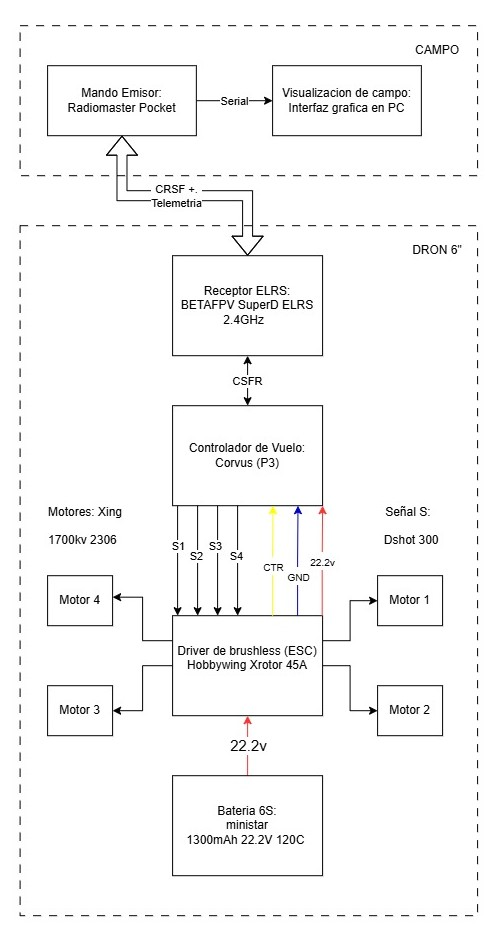
\includegraphics[width=0.6\linewidth]{Diagrama de Bloques P4.jpg}
    \caption{diagrama en bloques}
    \label{fig:diagrama_bloques}
\end{figure}

\begin{itemize}
    \item Segmento de campo
    \begin{itemize}
        \item Radiomaster Pocket (mando emisor).
    Se comunica con el PC de visualización mediante enlace serie UART sobre USB,
    empleando el protocolo de telemetría de EdgeTX.

        \item Módulo TX ELRS (interno al emisor).
    Establece el enlace aéreo con el receptor mediante ExpressLRS en la banda de
    2.4\,GHz, sobre modulación LoRa y con comunicación bidireccional.

        \item PC de visualización de campo.
    Recibe los datos del emisor por puerto serie sobre USB y los presenta en la
    interfaz gráfica.
    \end{itemize}

     \item Segmento aéreo
     \begin{itemize}
       \item Receptor BETAFPV SuperD ELRS 2.4\,GHz.
    Emplea ExpressLRS 2.4\,GHz en el enlace con el emisor y CRSF sobre UART a
    420\,kbaud en la conexión a bordo con el controlador de vuelo.

        \item Controlador de vuelo Corvus (P3).
    Recibe los canales de control por CRSF (UART) desde el receptor y genera las
    señales de mando hacia el ESC en protocolo DShot 300.

        \item Driver brushless Hobbywing XRotor 45A.
    Recibe las cuatro señales DShot 300 por las entradas S1--S4 y entrega a los
    motores una conmutación trifásica. Comparte con el controlador de vuelo la
    línea CTR de telemetría y la referencia de masa (GND).

        \item Motores Xing 2306 1700\,KV ($\times$4).
    No emplean protocolo digital alguno: reciben directamente del ESC la
    excitación trifásica conmutada.

        \item Batería Ministar 6S 1300\,mAh.
    Alimenta el ESC en corriente continua a 22{,}2\,V, sin protocolo de
    comunicación asociado.
    \end{itemize}
    \item Observaciones sobre los enlaces:

El enlace CRSF entre el receptor y el controlador de vuelo es bidireccional
sobre un único par TX/RX: transporta los canales de control hacia el controlador
y devuelve al emisor la telemetría (tensión de batería, RSSI y \textit{link
quality}) a través del propio enlace ExpressLRS. La línea CTR corresponde a la
telemetría del ESC hacia el controlador, que según el \textit{firmware} del
variador puede implementarse como telemetría serie a 115\,200\,baud o como DShot
bidireccional sobre las mismas líneas de señal, sin necesidad de un conductor
adicional. Las conexiones de potencia (22{,}2\,V y GND) no constituyen un
protocolo de comunicación, pero se incluyen por aparecer como enlaces explícitos
entre bloques del diagrama.

\end{itemize}

\subsection{Flujo del programa}

    % ---
    \begin{figure}[H]
    \centering
    % --- Columna de la Imagen ---
    \begin{minipage}[c]{0.48\textwidth}
        \centering
        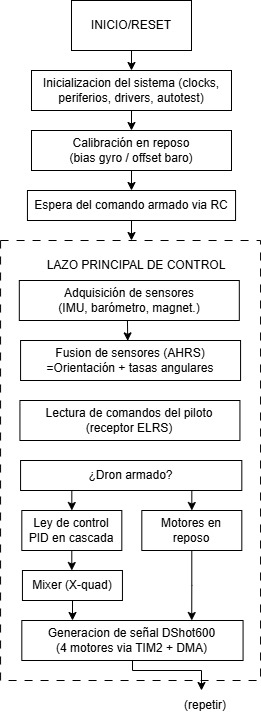
\includegraphics[width=0.9\linewidth]{Flujo dr programa.jpg}
        \caption{Flujo de programa}
        \label{fig:flujo_programa}
    \end{minipage}% <-- Este símbolo de porcentaje es clave para evitar espacios fantasma
    \hfill
    % --- Columna del Texto ---
    \begin{minipage}[c]{0.48\textwidth}
        El firmware del controlador de vuelo se estructura en dos fases. La fase de inicialización se ejecuta una única vez tras el reset del microcontrolador y configura los relojes, los periféricos (SPI, I²C, UART, USB, TIM2 con DMA), inicializa los drivers de cada sensor verificando su identidad, y realiza una calibración estática para estimar el bias del giroscopio y el offset de presión atmosférica del barómetro. A continuación, el sistema queda a la espera de que el operador active el comando de armado desde la radio.

        La fase operativa consiste en un lazo de control que se ejecuta a frecuencia fija. Cada iteración adquiere las muestras de los sensores inerciales, fusiona la información para obtener una estimación de la orientación y las velocidades angulares, lee los comandos enviados por el piloto desde el receptor ELRS, y decide en función del estado de armado si aplicar la ley de control en cascada (lazo externo de actitud + lazo interno de velocidad angular) o mantener los motores en reposo. La salida del controlador se convierte mediante el mezclador en cuatro valores de empuje individuales que se envían a los ESCs mediante el protocolo DShot300.
    \end{minipage}
\end{figure}
  % ---
\subsection{Product Breakdown Structure (PBS)}
\begin{figure}[H]
    \centering
    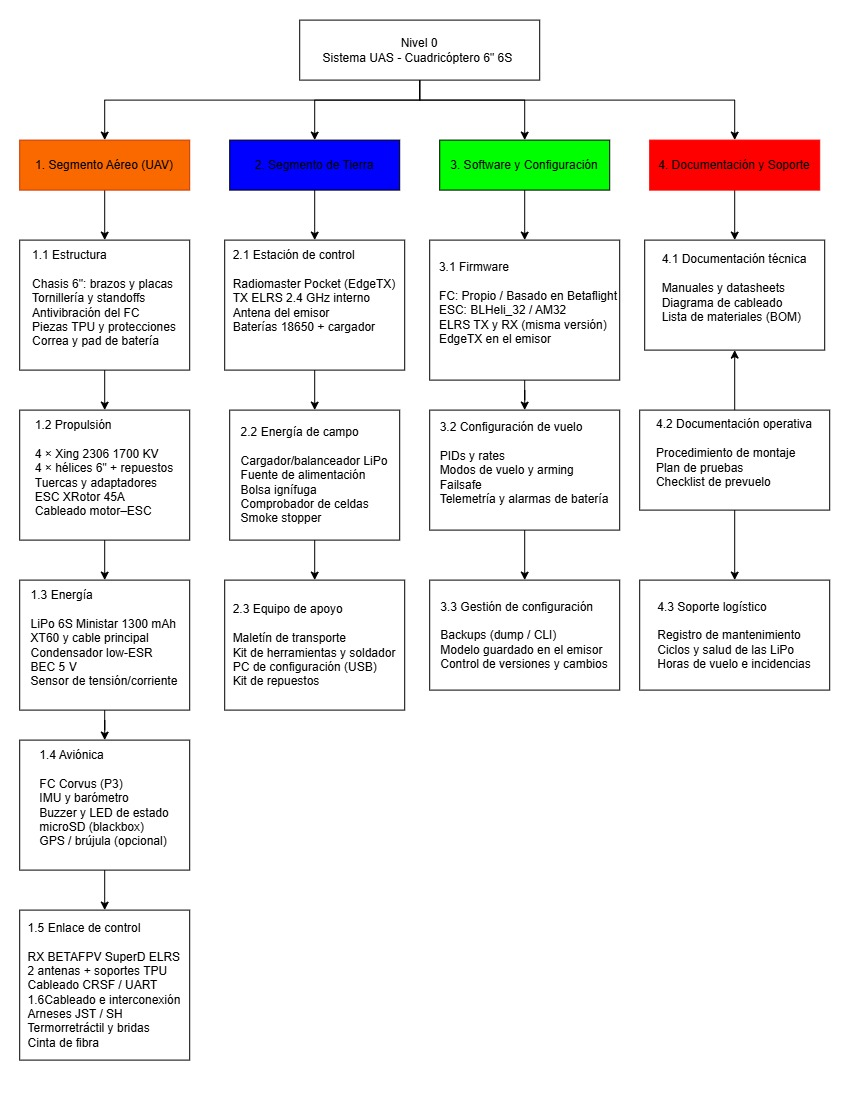
\includegraphics[width=0.9\linewidth]{PBS P4 .jpg}
    \caption{Product Breakdown Structure}
    \label{fig:pbs}
\end{figure}


% 7. Diseños
\section{Diseños}
\subsection{Diseño Electrónico}
El diseño del hardware se divide en la captura esquemática y el ruteo de la placa de circuito impreso (PCB). El esquemático detalla las interconexiones entre el STM32F405RGT6, los sensores (IMU LSM6DSV16X, Barómetro BMP388) y los periféricos externos, prestando especial atención a la arquitectura de alimentación.

\subsubsection{Esquemáticos}
Las Figuras~\ref{fig:esq_mcu} a~\ref{fig:esq_usb} presentan la captura esquemática completa, organizada por bloques funcionales: microcontrolador, sensores, regulación de potencia, e interfaz USB tipo C con conectores externos.

\begin{figure}[H]
    \centering
    \includegraphics[width=\linewidth, height=0.42\textheight, keepaspectratio, page=2]{Esquematico_1.pdf}
    \caption{MCU STM32F405RGT6.}
    \label{fig:esq_mcu}
\end{figure}

\begin{figure}[H]
    \centering
    \includegraphics[width=\linewidth, height=0.42\textheight, keepaspectratio, page=3]{Esquematico_1.pdf}
    \caption{Sensores (IMU, barómetro y magnetómetro).}
    \label{fig:esq_sensores}
\end{figure}

\begin{figure}[H]
    \centering
    \includegraphics[width=\linewidth, height=0.42\textheight, keepaspectratio, page=4]{Esquematico_1.pdf}
    \caption{Regulación de potencia.}
    \label{fig:esq_potencia}
\end{figure}

\begin{figure}[H]
    \centering
    \includegraphics[width=\linewidth, height=0.42\textheight, keepaspectratio, page=5]{Esquematico_1.pdf}
    \caption{USB tipo C y conectores externos.}
    \label{fig:esq_usb}
\end{figure}

\subsubsection{Diseño de la PCB}
El layout de la placa se diseñó en un formato estándar de 40$\times$40~mm con orificios de montaje de 30$\times$30~mm. Se utilizó una configuración de seis capas para aislar las señales de alta frecuencia (como el bus SDIO y USB) de los planos de potencia. En la Figura~\ref{fig:capas_pcb} se aprecian las seis capas de cobre del diseño y en la Tabla~\ref{tab:capas_pcb} la distribución de componentes y funciones por capa.

\begin{figure}[htbp]
    \centering
    \begin{subfigure}[b]{0.48\textwidth}
        \centering
        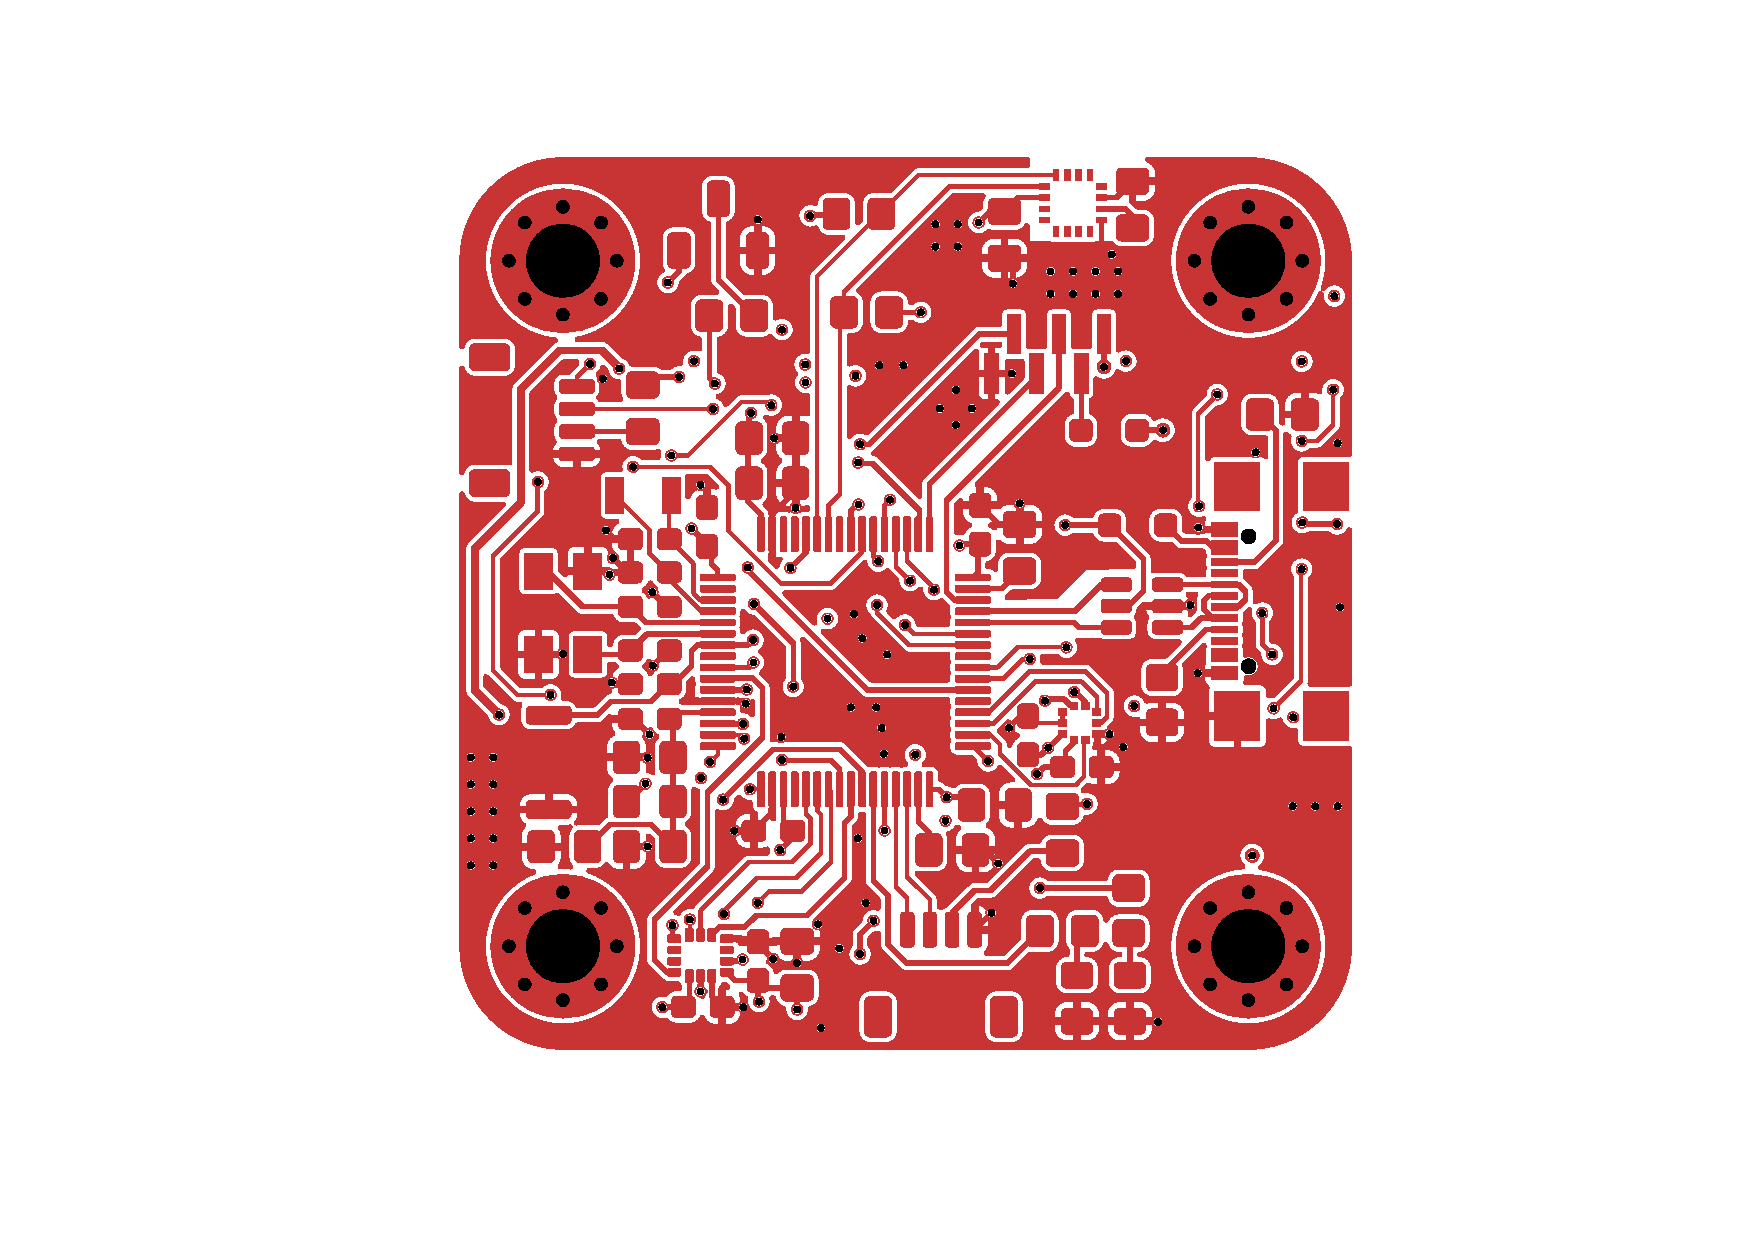
\includegraphics[width=\linewidth]{F.pdf}
        \caption{Top Copper (F.Cu)}
    \end{subfigure}
    \hfill
    \begin{subfigure}[b]{0.48\textwidth}
        \centering
        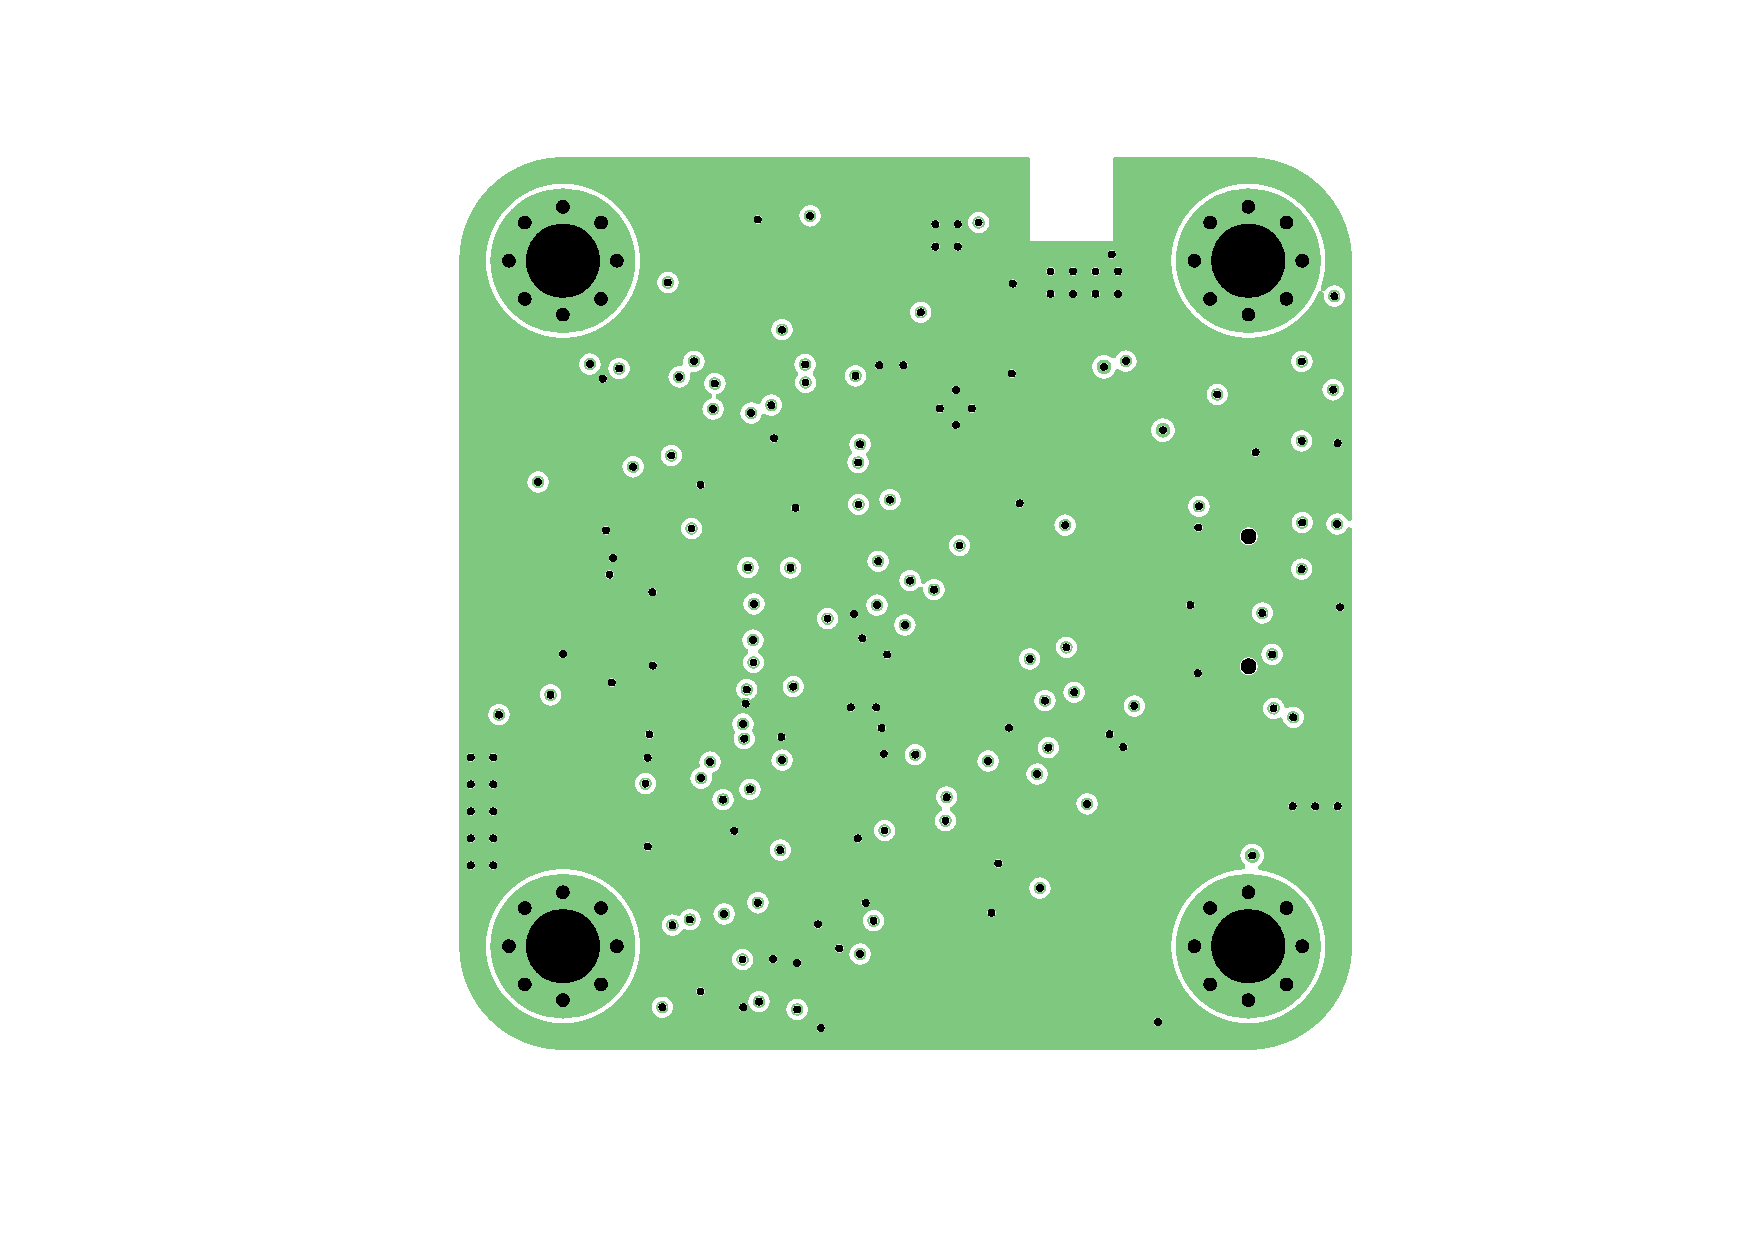
\includegraphics[width=\linewidth]{IN1.pdf}
        \caption{In1.Cu (Internal 1)}
    \end{subfigure}

    \vspace{10pt}

    \begin{subfigure}[b]{0.48\textwidth}
        \centering
        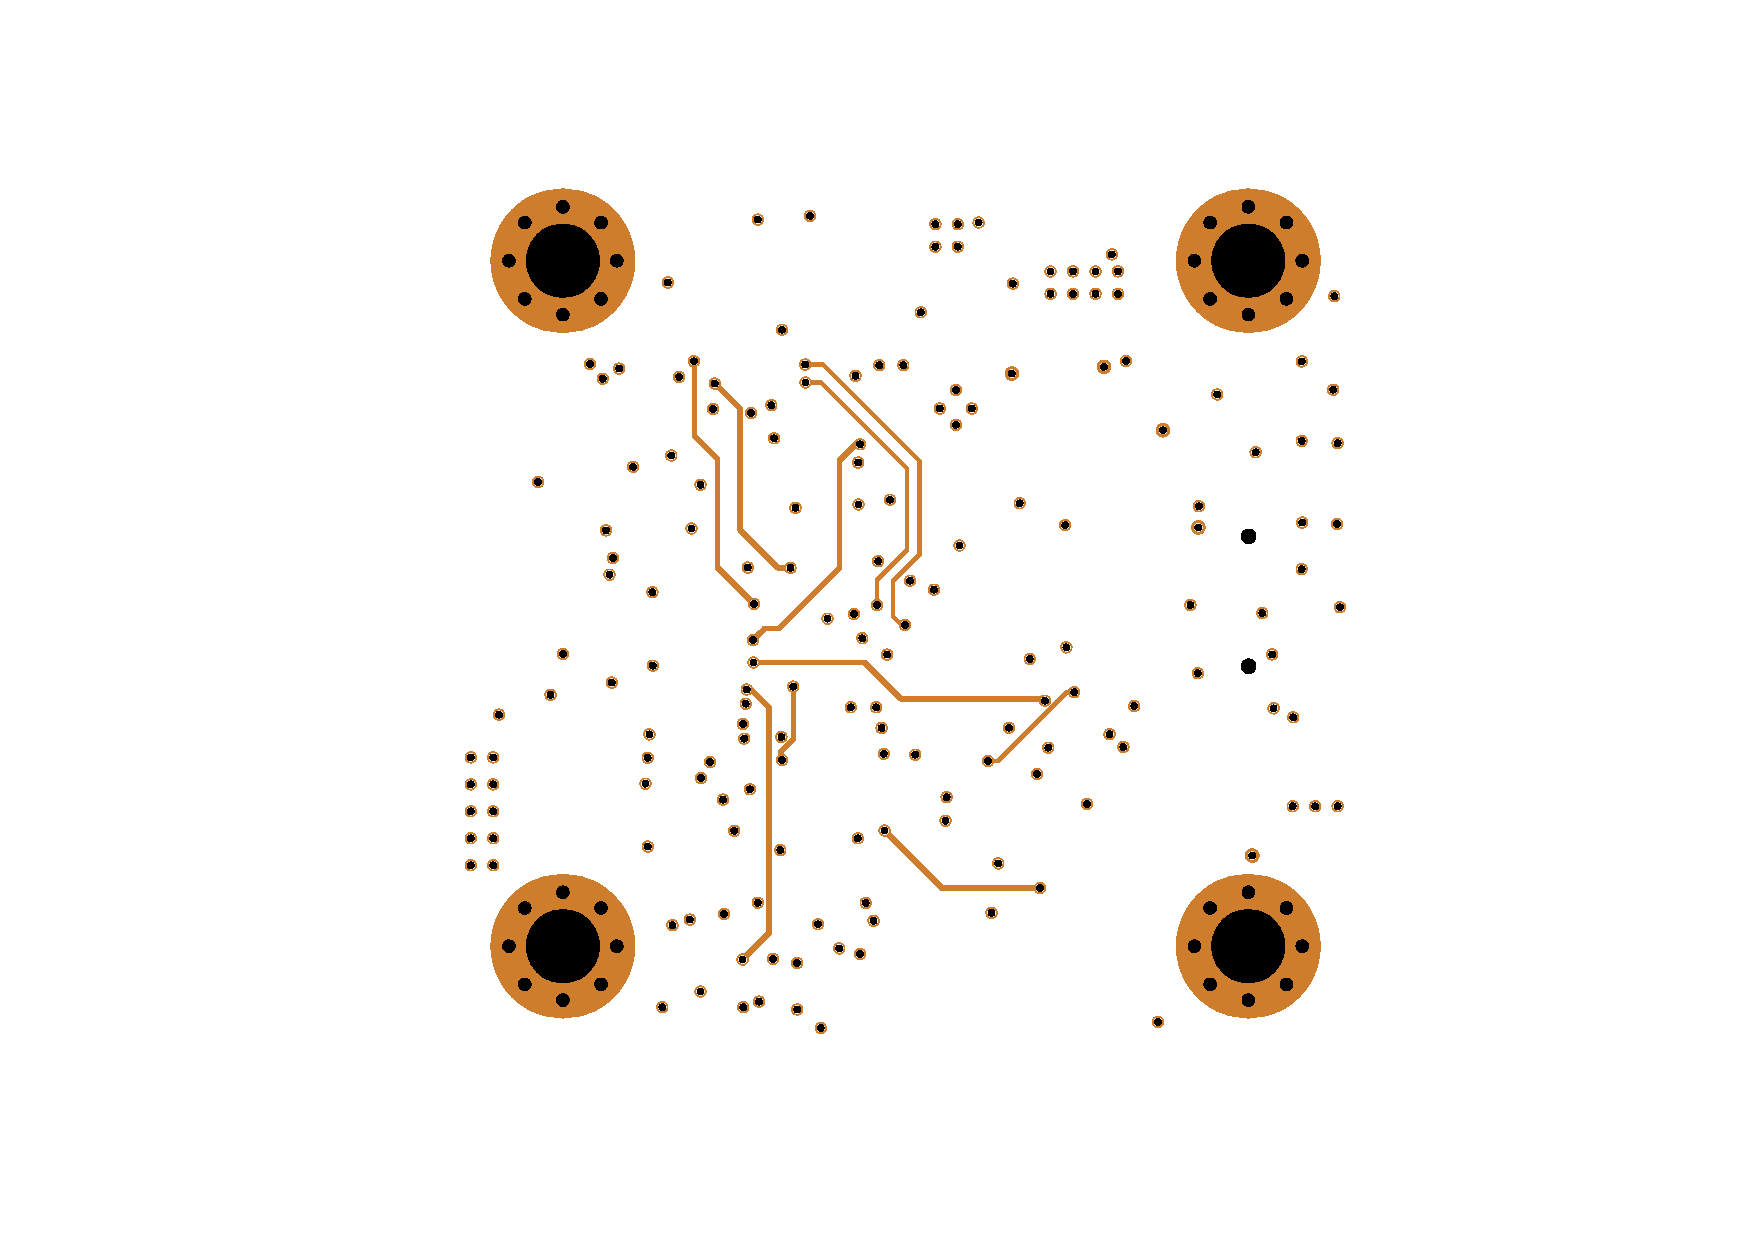
\includegraphics[width=\linewidth]{IN2.pdf}
        \caption{In2.Cu (Internal 2)}
    \end{subfigure}
    \hfill
    \begin{subfigure}[b]{0.48\textwidth}
        \centering
        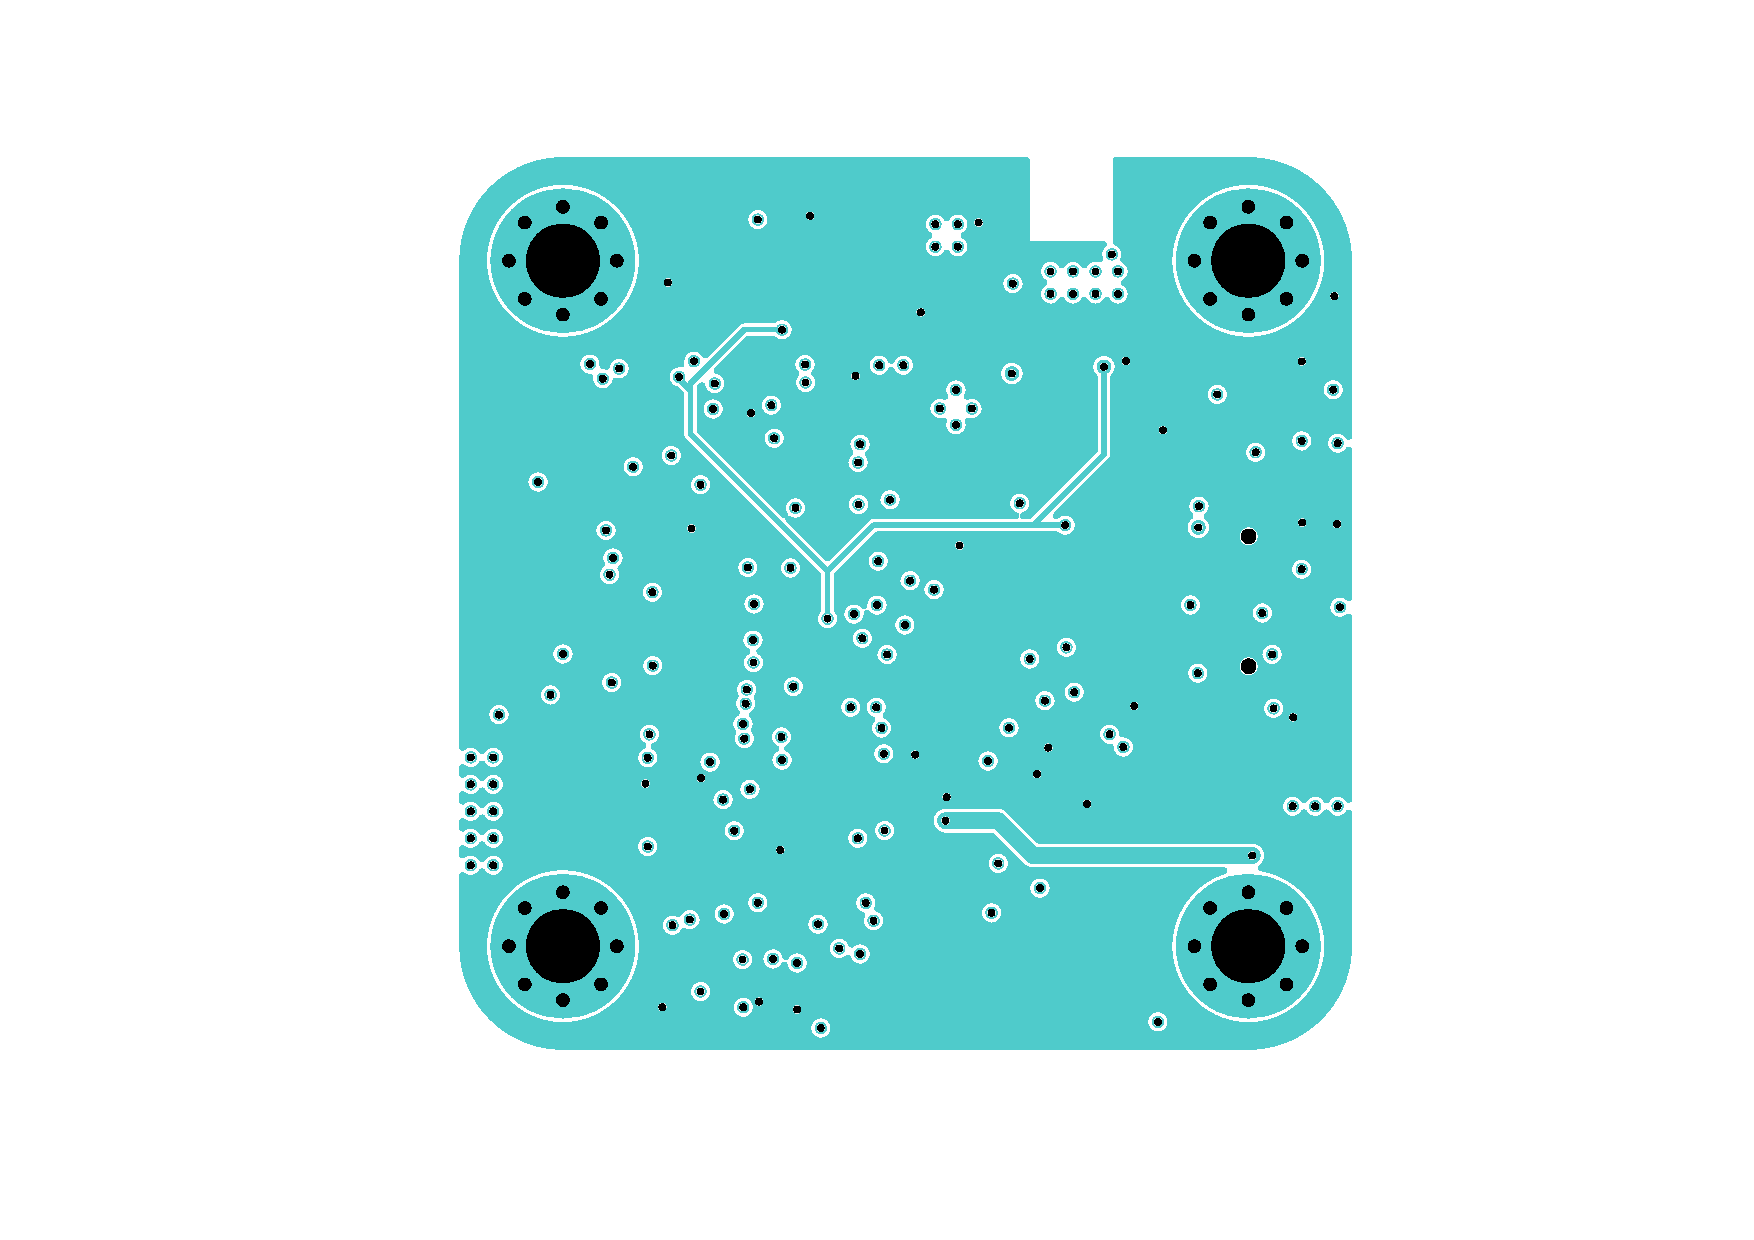
\includegraphics[width=\linewidth]{IN3.pdf}
        \caption{In3.Cu (Internal 3)}
    \end{subfigure}

    \vspace{10pt}

    \begin{subfigure}[b]{0.48\textwidth}
        \centering
        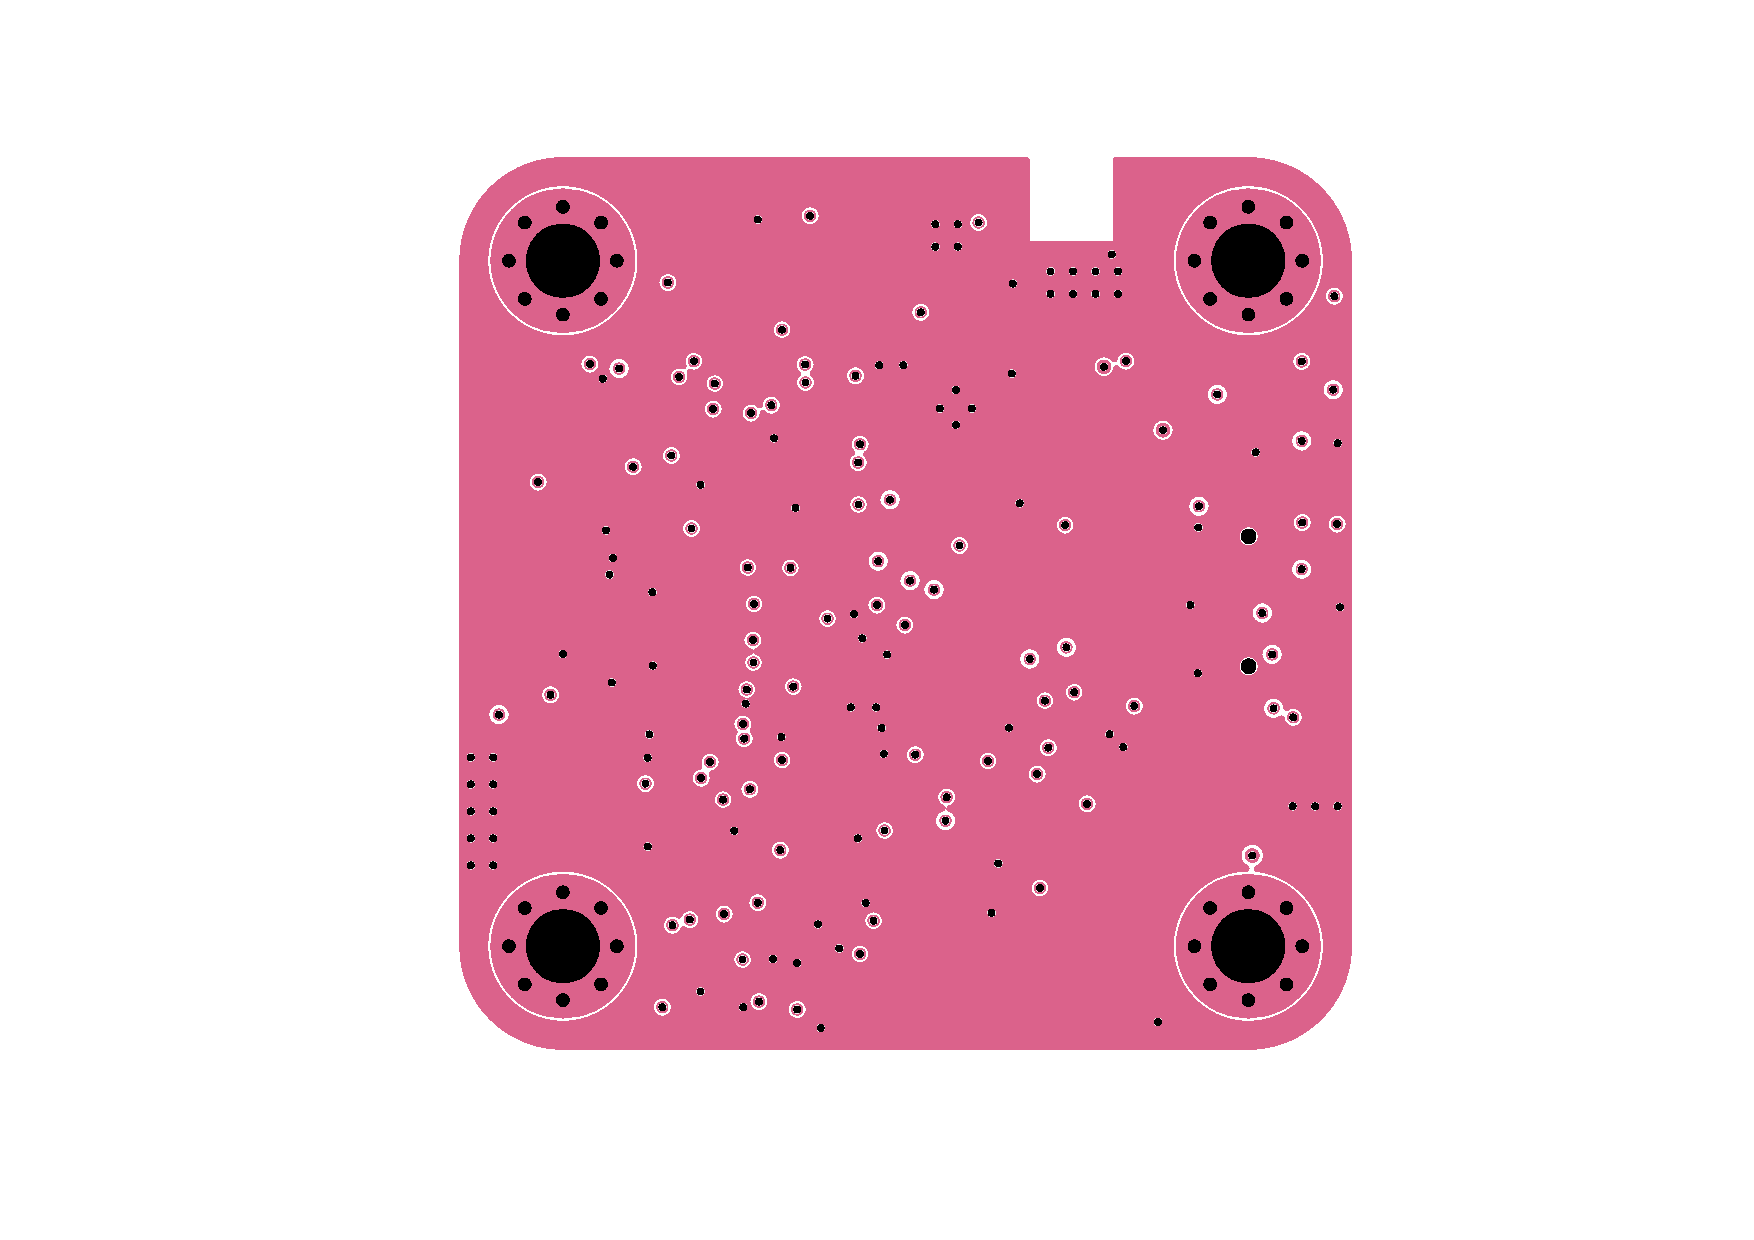
\includegraphics[width=\linewidth]{IN4.pdf}
        \caption{In4.Cu (Internal 4)}
    \end{subfigure}
    \hfill
    \begin{subfigure}[b]{0.48\textwidth}
        \centering
        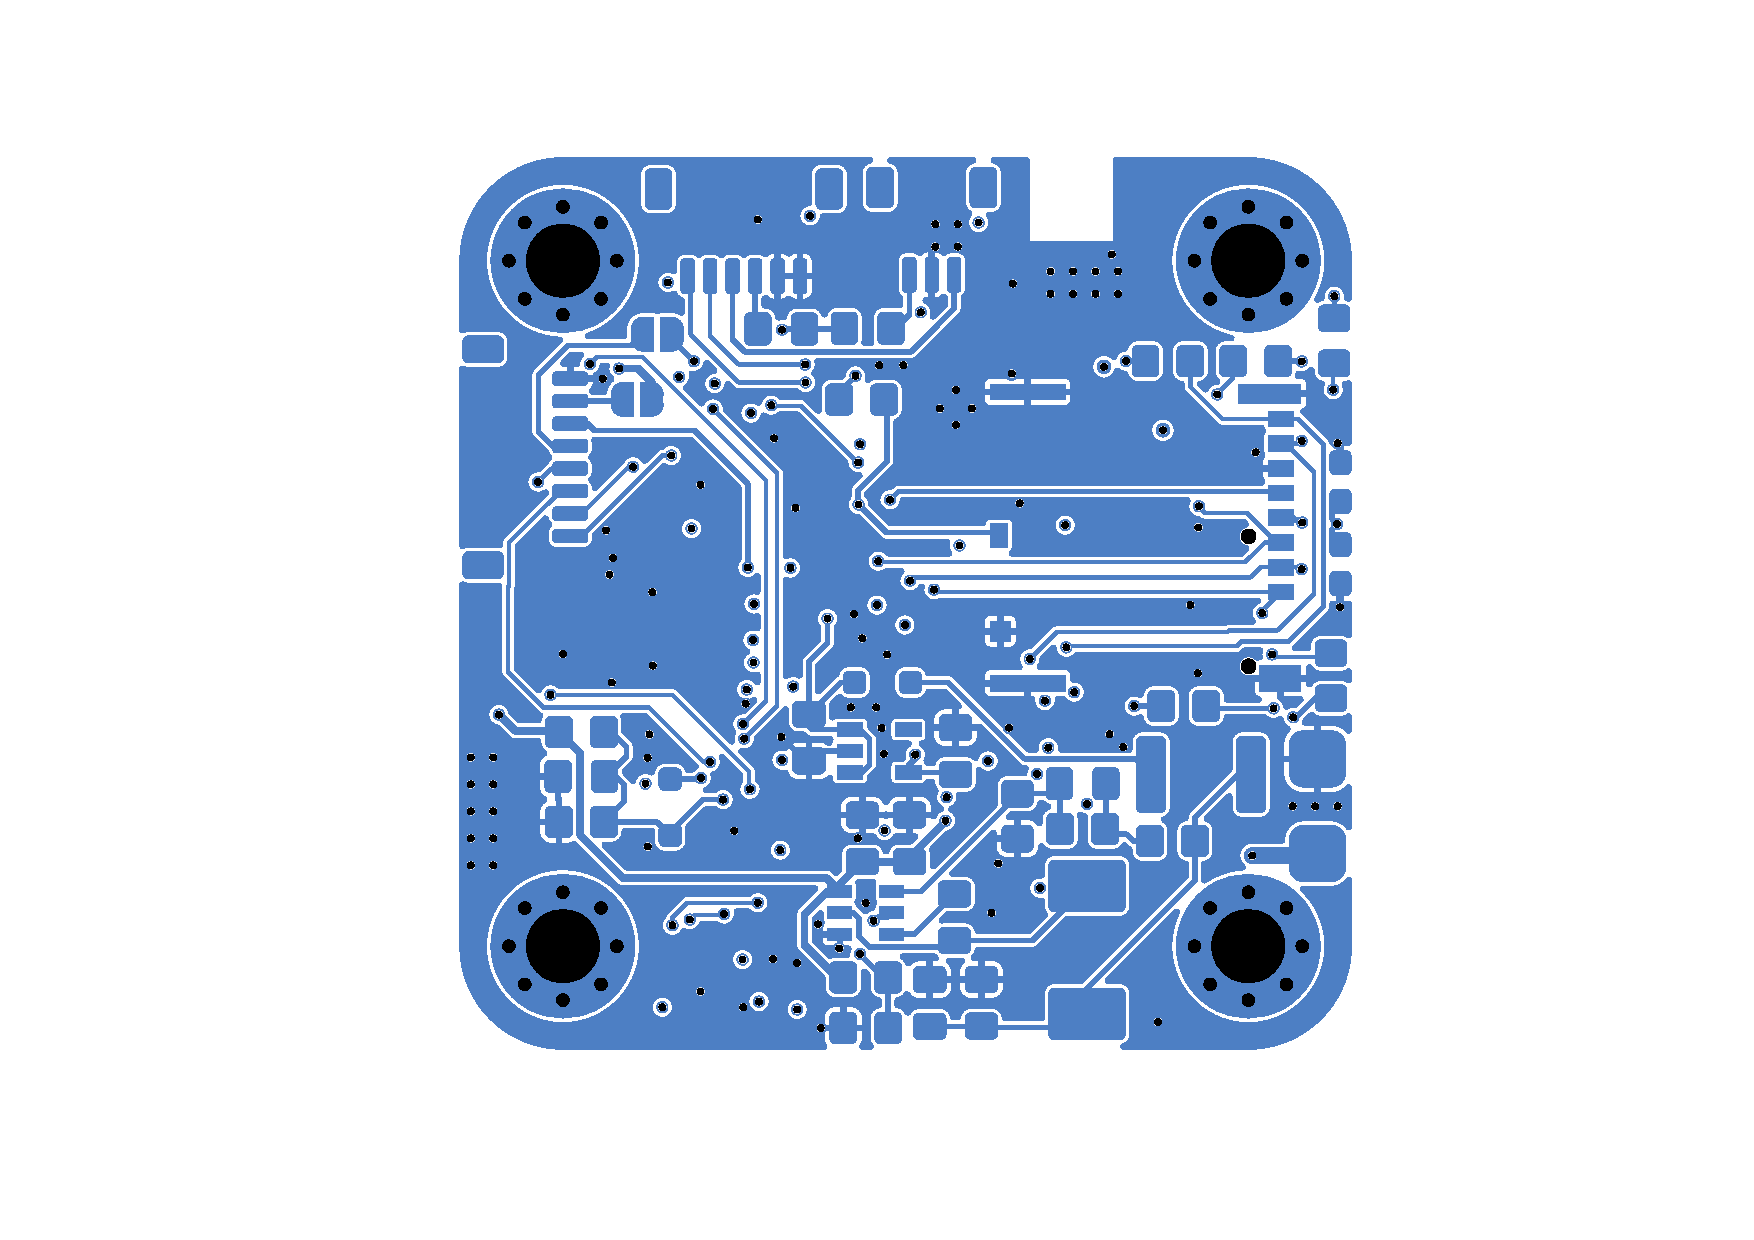
\includegraphics[width=\linewidth]{B.pdf}
        \caption{Bottom Copper (B.Cu)}
    \end{subfigure}

    \caption{Visualización de las 6 capas del diseño de la PCB.}
    \label{fig:capas_pcb}
\end{figure}

\subsubsection{Ensamblado y retrabajo}
\begin{figure}[H]
    \centering
    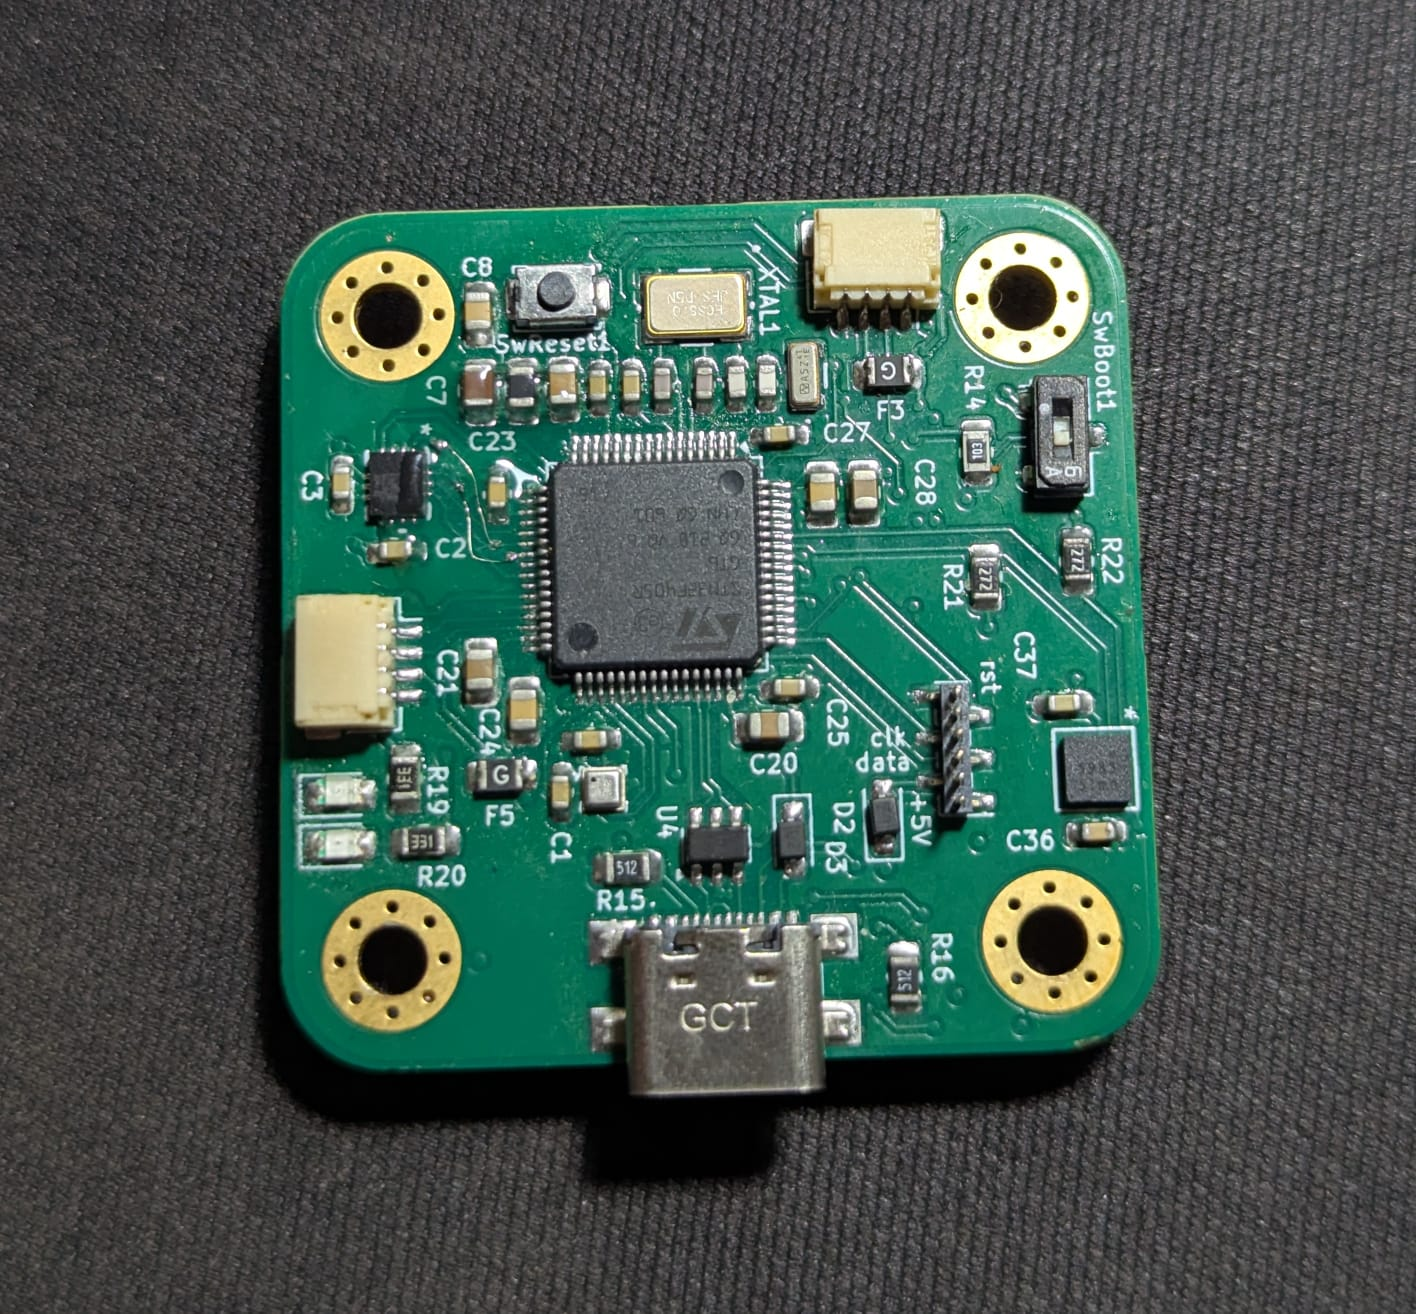
\includegraphics[width=12cm, height=8cm, keepaspectratio]{pcb.jpeg}
    \caption{PCB ensamblada del controlador de vuelo CORVUS.}
    \label{fig:pcb_ensamblada}
\end{figure}

Tras el ensamblado se requirió un retrabajo sobre la IMU LSM6DSV16X: las conexiones afectadas se puentearon con conductores unifilares para restablecer la continuidad de las pistas. Una vez verificadas las uniones, se aplicó esmalte aislante sobre el puenteo y, posteriormente, un recubrimiento de curado UV para proteger mecánicamente la zona, evitar cortocircuitos y reducir el riesgo de degradación por vibración en vuelo.

\begin{table}[htbp]
\centering
\caption{Distribución de componentes por capa de la PCB}
\label{tab:capas_pcb}
\renewcommand{\arraystretch}{1.3}
\setlength{\tabcolsep}{10pt}
\begin{tabular}{@{}c p{11cm}@{}}
\toprule
\rowcolor{gray!20}
\textbf{Capa} & \textbf{Componentes / Función} \\
\midrule
\textbf{Capa 1} & USB, IMU, barómetro, magnetómetro, STM y cristales \\
\textbf{Capa 2} & Plano de GND \\
\textbf{Capa 3} & Señales \\
\textbf{Capa 4} & Plano de alimentación de 3.3V y 5V \\
\textbf{Capa 5} & Plano de GND \\
\textbf{Capa 6} & LDO, BUCK y MicroSD \\
\bottomrule
\end{tabular}
\end{table}

\subsection{Diseño Mecánico}

\begin{figure}[H]
    \centering
    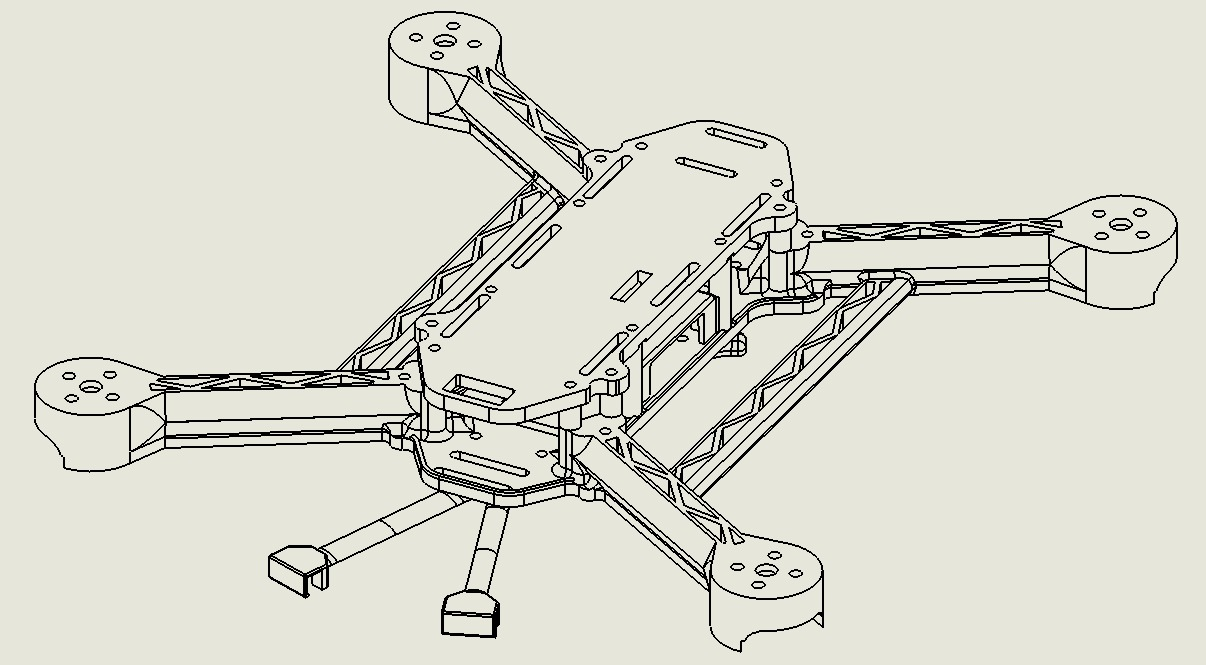
\includegraphics[width=12cm, height=8cm, keepaspectratio]{Ensamble_V2.png}
    \caption{Diseño ensamblado del dron (versión 2): cuerpo y brazos en una sola pieza, con los soportes entre brazos y el acople de aterrizaje y mástil.}
    \label{fig:ensamble}
\end{figure}
\begin{figure}[H]
    \centering
    \begin{subfigure}[b]{0.48\textwidth}
        \centering
        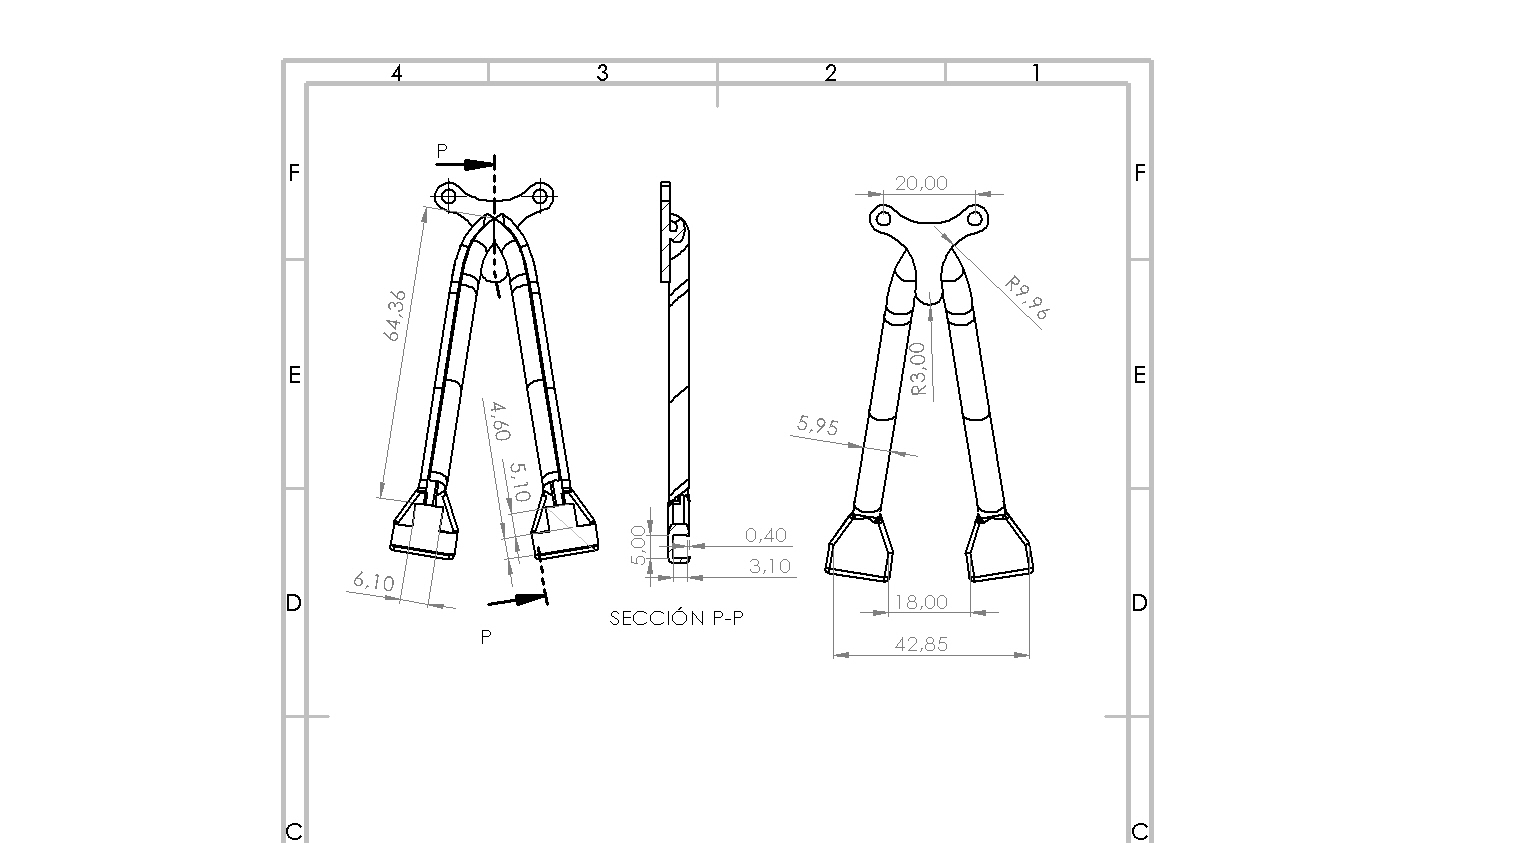
\includegraphics[trim={6.0cm 0cm 7.8cm 0cm}, clip, width=7cm, height=16cm, keepaspectratio]{Soporte_ELRS.JPG}
        \caption{Soporte de la Antena ELRS}
        \label{fig:soporte_elrs}
    \end{subfigure}
    \hfill
    \begin{subfigure}[b]{0.48\textwidth}
        \centering
        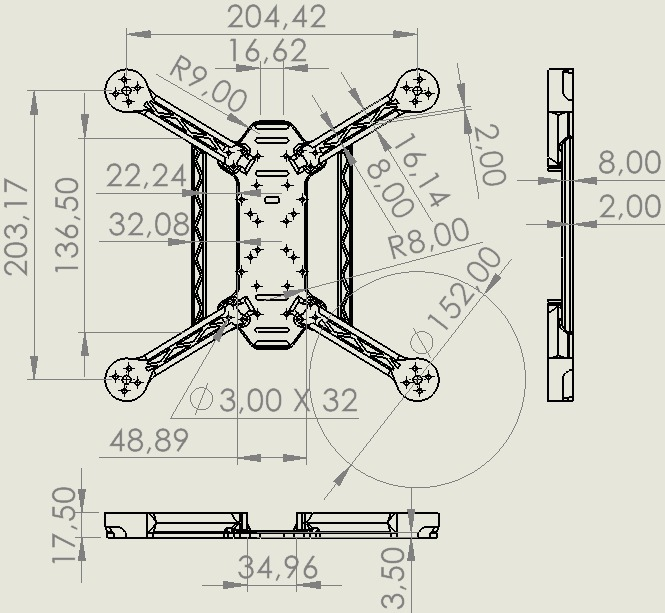
\includegraphics[width=7cm, height=16cm, keepaspectratio]{Estructura_cuerpo_brazos.png}
        \caption{Dibujo mecánico del cuerpo con los brazos (pieza única)}
        \label{fig:base}
    \end{subfigure}
    \caption{Soporte ELRS y dibujo mecánico del cuerpo con los brazos.}
    \label{fig:elrs_base}
\end{figure}
\begin{figure}[H]
    \centering
    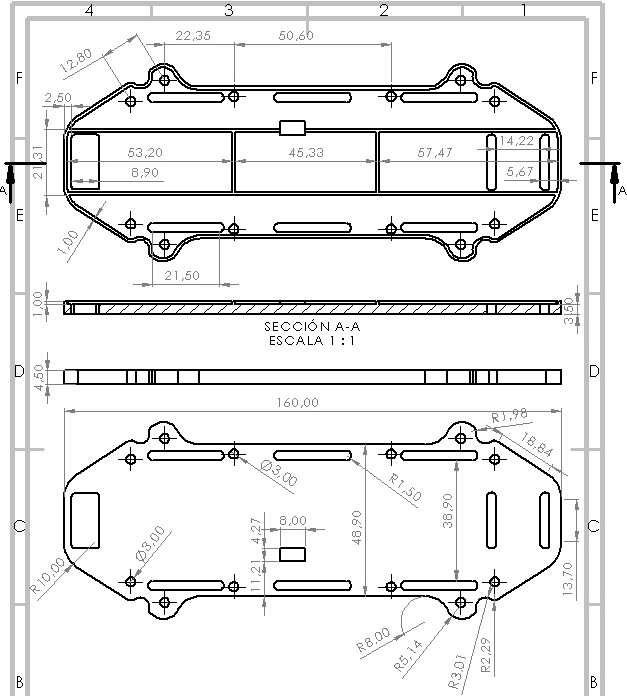
\includegraphics[width=12cm, height=8cm, keepaspectratio]{Tapa_FromScratch.JPG}
    \caption{Dibujo Mecánico de la Tapa del dron}
    \label{fig:tapa}
\end{figure}
\begin{figure}[H]
    \centering
    \begin{subfigure}[b]{0.48\textwidth}
        \centering
        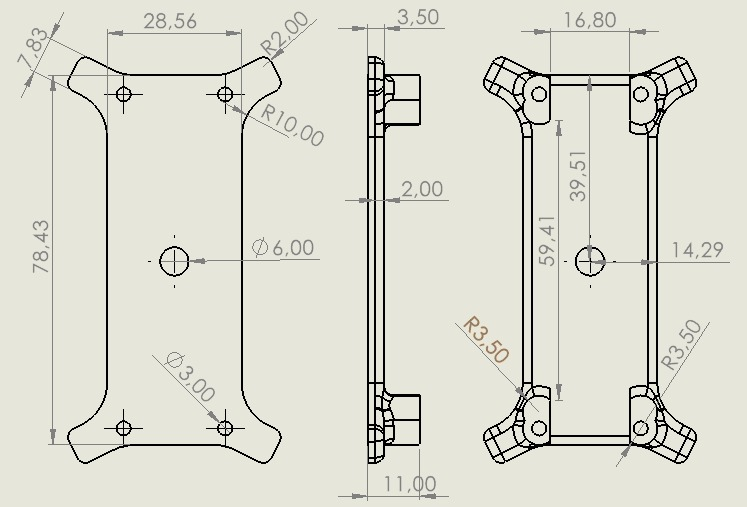
\includegraphics[width=7cm, height=6cm, keepaspectratio]{Estructura_tapa_soporte.png}
        \caption{Dibujo mecánico del acople para el apoyo de aterrizaje y el mástil}
        \label{fig:brazo}
    \end{subfigure}
    \hfill
    \begin{subfigure}[b]{0.48\textwidth}
        \centering
        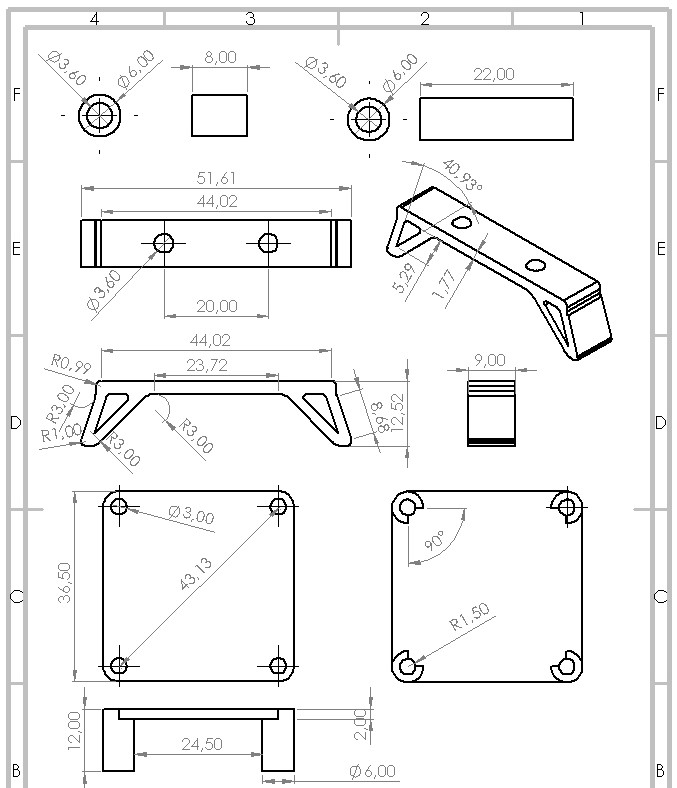
\includegraphics[width=7cm, height=6cm, keepaspectratio]{Soportes.JPG}
        \caption{Dibujo Mecánico de los soportes internos y externos del dron}
        \label{fig:soportes}
    \end{subfigure}
    \caption{Dibujos mecánicos del acople de aterrizaje y mástil y de los soportes internos y externos.}
    \label{fig:brazo_soportes}
\end{figure}

La estructura tomó como referencia el Groover 280 v1.1 Quadcopter Frame, un chasis de configuración true X para hélices de 6 pulgadas con herencia de vuelo demostrada, modificado en esta versión y con numerosas uniones que le dan un carácter modular (la circunferencia de $\varnothing 152$~mm de la Figura~\ref{fig:base} representa la hélice). Su geometría simétrica iguala los momentos de inercia en los ejes de alabeo y cabeceo, lo que simplifica el modelo dinámico del vehículo y facilita la sintonización del controlador. El cuerpo ocupa $204{,}42 \times 203{,}17$~mm en planta y tiene 17,5~mm de alto, con 32 agujeros de $\varnothing 3$~mm para el montaje del stack, los motores y los accesorios.

\paragraph{Cambios respecto de la versión anterior.} La primera versión estaba formada por piezas separadas: la base, la tapa inferior y los brazos. En esta versión se imprimió en \textbf{una sola pieza la tapa inferior junto con los brazos}, que se unieron para obtener mayor rigidez general. Además, ahora se utilizan \textbf{soportes entre brazos} (los travesaños laterales que se ven a ambos lados del cuerpo en la Figura~\ref{fig:base}): al vincular el brazo delantero con el trasero de cada lado forman una estructura cerrada que evita que cada brazo flexione y vibre de forma independiente, con lo que aumenta la rigidez y disminuyen las vibraciones de los motores que llegan a la IMU, que es lo que más degrada la estimación de actitud y el lazo de control. La pieza se imprimió en \textbf{PETG con relleno del 100\,\%}, material con buena resistencia a impactos y algo de amortiguamiento, adecuado para una estructura que debe soportar golpes y vibración.

También se agregó una pieza nueva, el \textbf{acople para el apoyo de aterrizaje y para el mástil} (Figura~\ref{fig:brazo}): una placa de 2~mm de espesor y $78{,}43 \times 28{,}56$~mm con cuatro agujeros de $\varnothing 3$~mm y un pasaje central de $\varnothing 6$~mm, cuyo marco posterior de $59{,}41 \times 16{,}80$~mm tiene cuatro ménsulas en las esquinas para fijar el apoyo de aterrizaje y el mástil del GPS.

\begin{figure}[H]
    \centering
    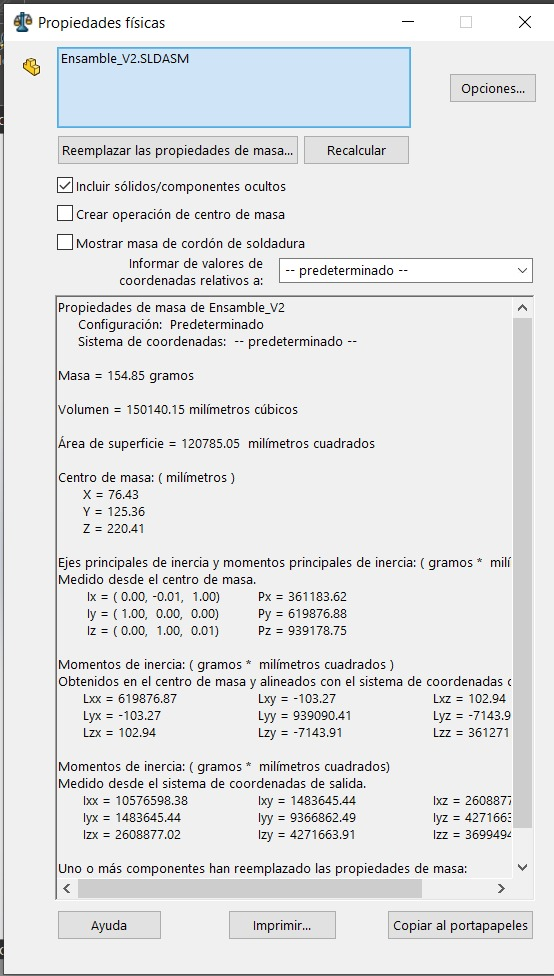
\includegraphics[height=12cm, keepaspectratio]{Propiedades_SolidWorks.png}
    \caption{Propiedades físicas del ensamble (\texttt{Ensamble\_V2}) obtenidas en SolidWorks.}
    \label{fig:propiedades_sw}
\end{figure}

\begin{table}[htbp]
\centering
\caption{Propiedades físicas del ensamble estructural (SolidWorks, PETG 100\,\%)}
\label{tab:propiedades_sw}
\renewcommand{\arraystretch}{1.3}
\small
\begin{tabular}{@{}l r@{}}
\toprule
\rowcolor{gray!20}
\textbf{Propiedad} & \textbf{Valor} \\
\midrule
Masa & 154,85~g \\
Volumen & 150\,140~mm\textsuperscript{3} \\
Área de superficie & 120\,785~mm\textsuperscript{2} \\
Centro de masa (X, Y, Z) & 76,43;\ 125,36;\ 220,41~mm \\
Momentos principales de inercia & $3{,}61\times10^{-4}$;\ $6{,}20\times10^{-4}$;\ $9{,}39\times10^{-4}$~kg\,m\textsuperscript{2} \\
\bottomrule
\end{tabular}
\end{table}

La estructura pesa 154,85~g, alrededor del 17\,\% de la masa total estimada del dron (900~g). El mayor momento de inercia ($9{,}39\times10^{-4}$~kg\,m\textsuperscript{2}) corresponde al eje vertical (guiñada), como es de esperar en una estructura plana, y los otros dos, de $3{,}61\times10^{-4}$ y $6{,}20\times10^{-4}$~kg\,m\textsuperscript{2}, a los ejes de alabeo y cabeceo; estos valores se usan como punto de partida para el modelo dinámico y la sintonización del controlador.

\begin{figure}[H]
    \centering
    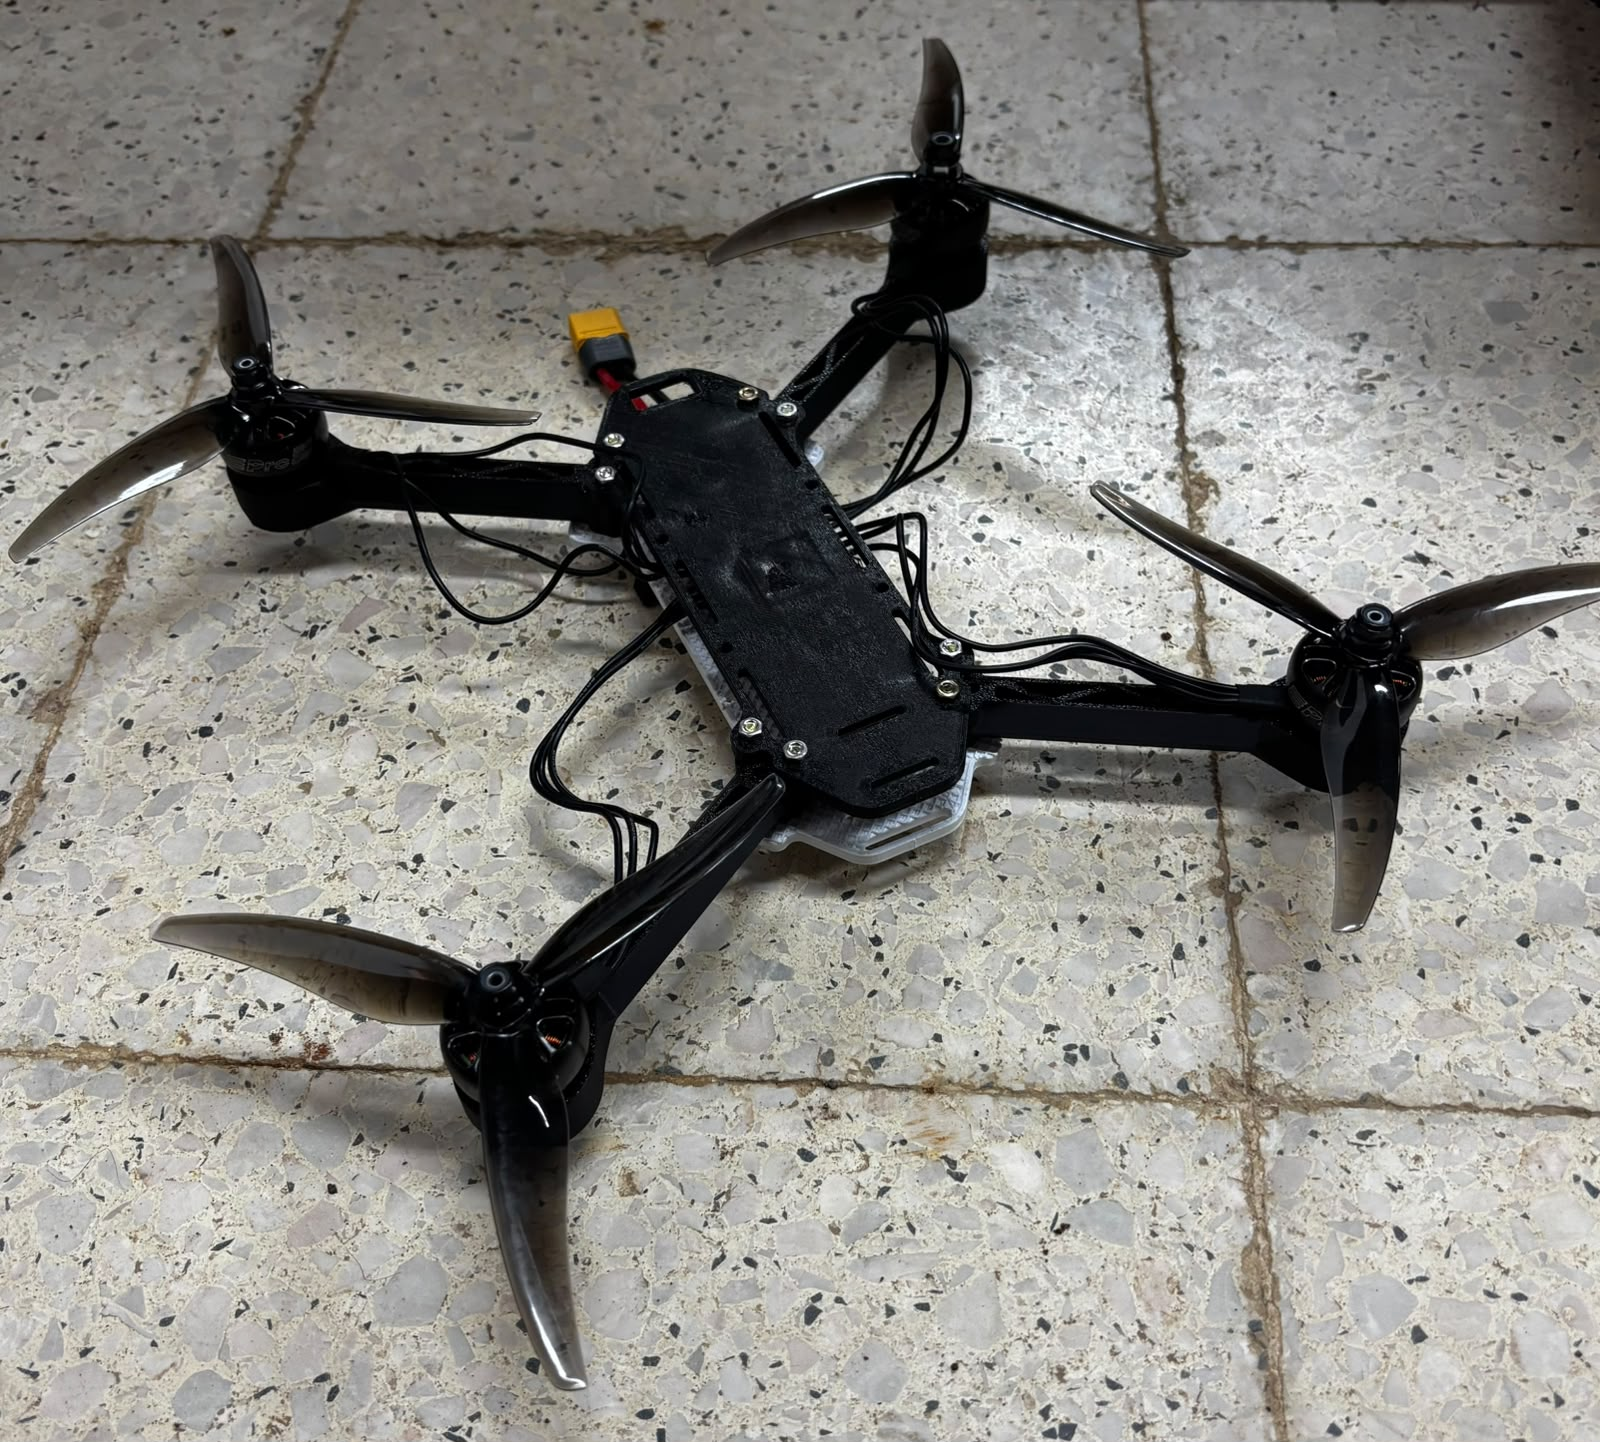
\includegraphics[width=12cm, height=8cm, keepaspectratio]{estructura.jpeg}
    \caption{Dron parcialmente montado sobre el chasis.}
    \label{fig:estructura}
\end{figure}

El ensamble se encuentra en fase de pruebas de resistencia y rigidez estructural. El objetivo de esta etapa es verificar que el chasis True~X sostenga el stack electrónico, los motores y la batería sin deformaciones excesivas ni holguras en las uniones, de modo que las vibraciones transmitidas a la IMU permanezcan dentro de un rango compatible con el control de vuelo.

\subsection{Diseño Interfaz}
En el diseño de la interfaz se tiene en cuenta el Giroscopio, acelerómetro, magnetómetro y barómetro, para tener una visualizacion de la orientación del dron con datos en tiempo real.

La interfaz es una estación de tierra web (GCS) que recibe la telemetría del dron en vuelo a través del enlace ELRS y la muestra en tiempo real; su funcionamiento se describe en la sección siguiente. Las Figuras~\ref{fig:gcs_general} a~\ref{fig:gcs_sistema} muestran su aspecto actual.

\begin{figure}[H]
    \centering
    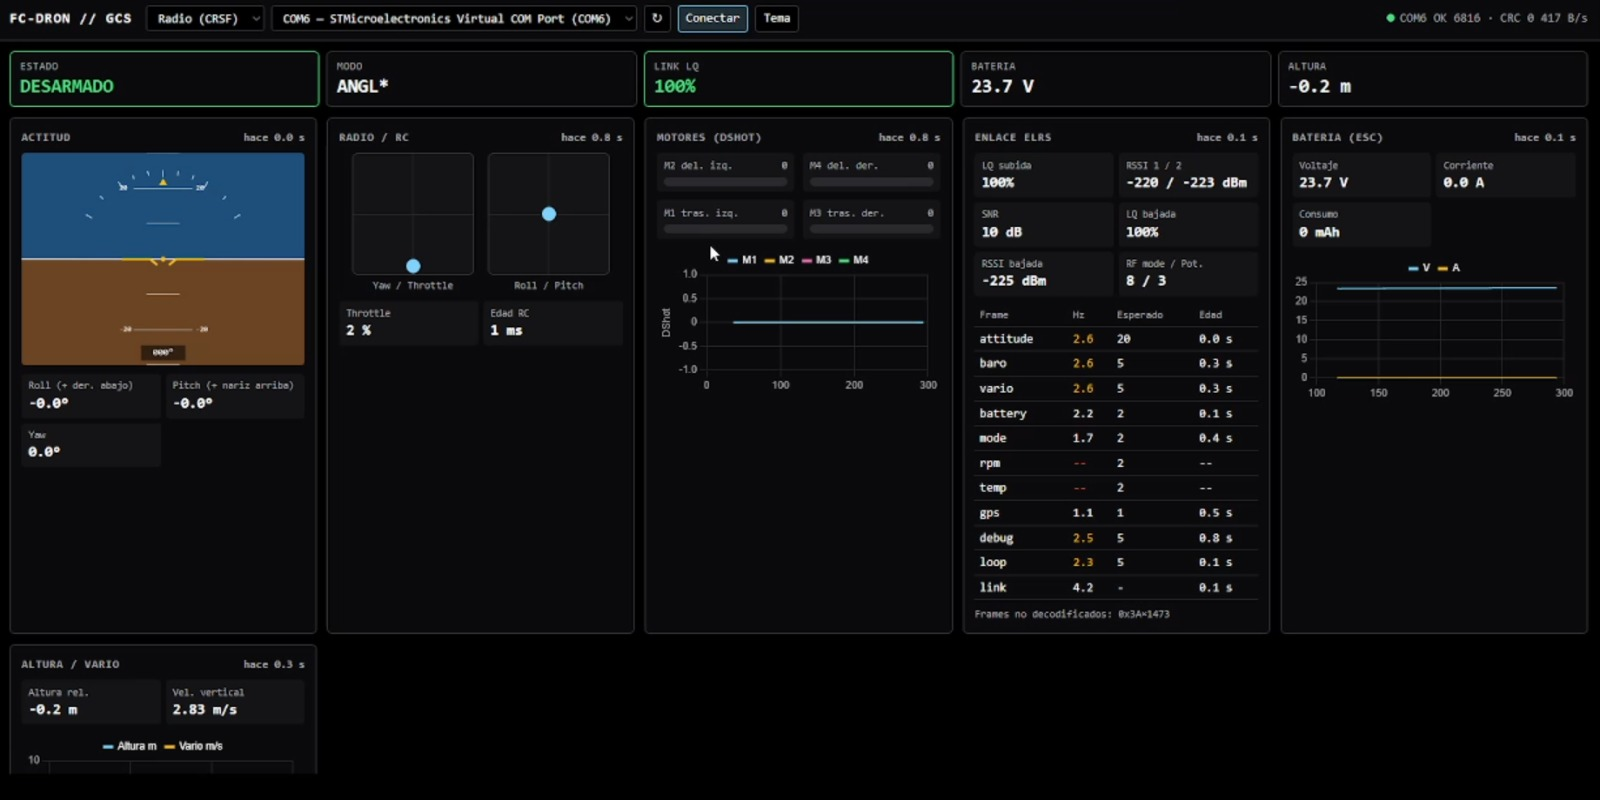
\includegraphics[width=1\linewidth]{GCS_general.png}
    \caption{GCS, vista general: estado de armado, modo, calidad del enlace, batería y altura; actitud, radio, motores, enlace ELRS con las tasas de cada frame, batería y altura.}
    \label{fig:gcs_general}
\end{figure}

\begin{figure}[H]
    \centering
    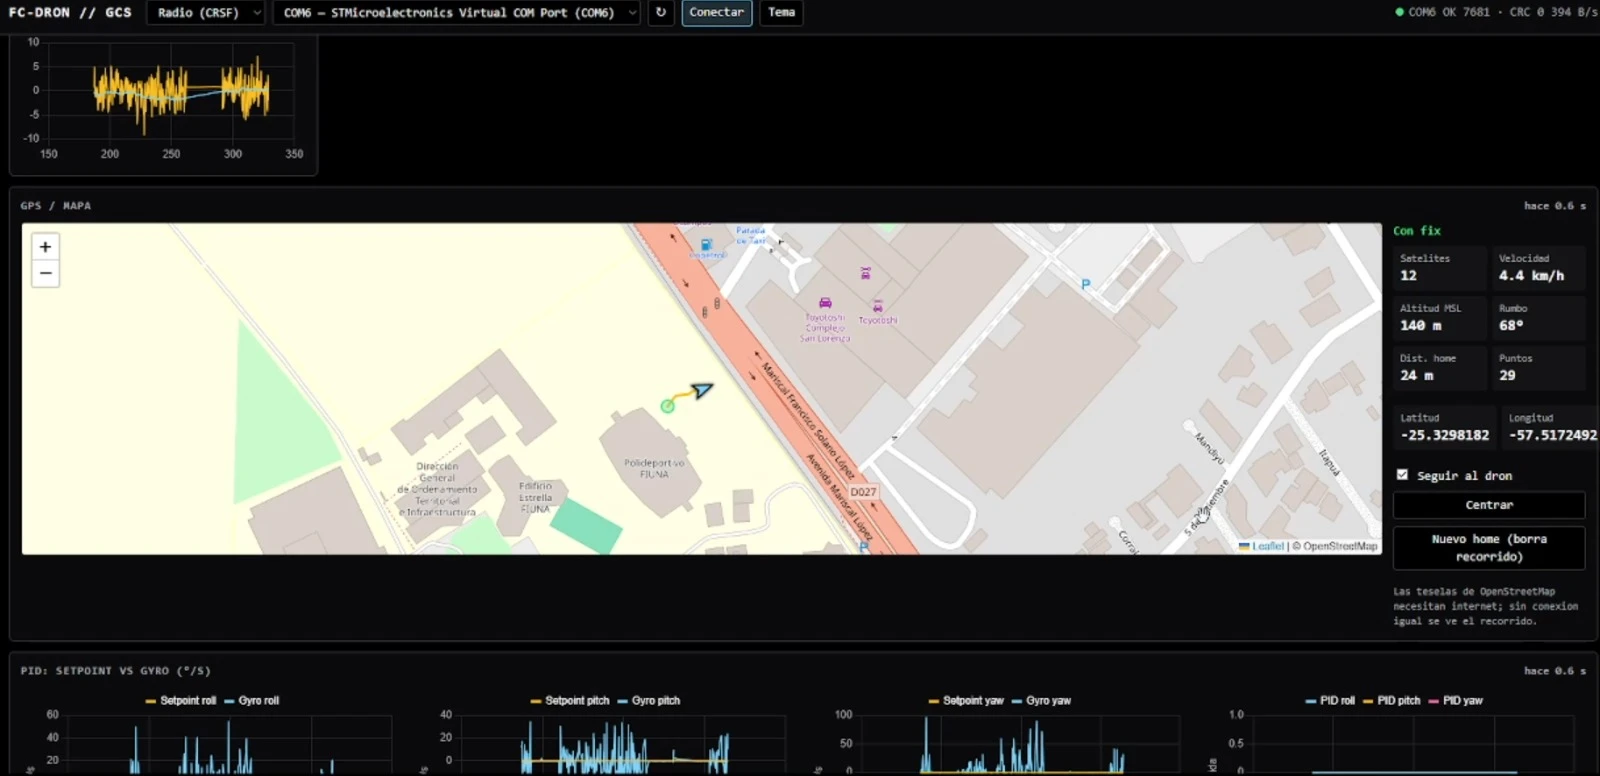
\includegraphics[width=1\linewidth]{GCS_mapa_gps.png}
    \caption{GCS, tarjeta GPS / Mapa y gráficos del PID (consigna contra giroscopio).}
    \label{fig:gcs_mapa}
\end{figure}

\begin{figure}[H]
    \centering
    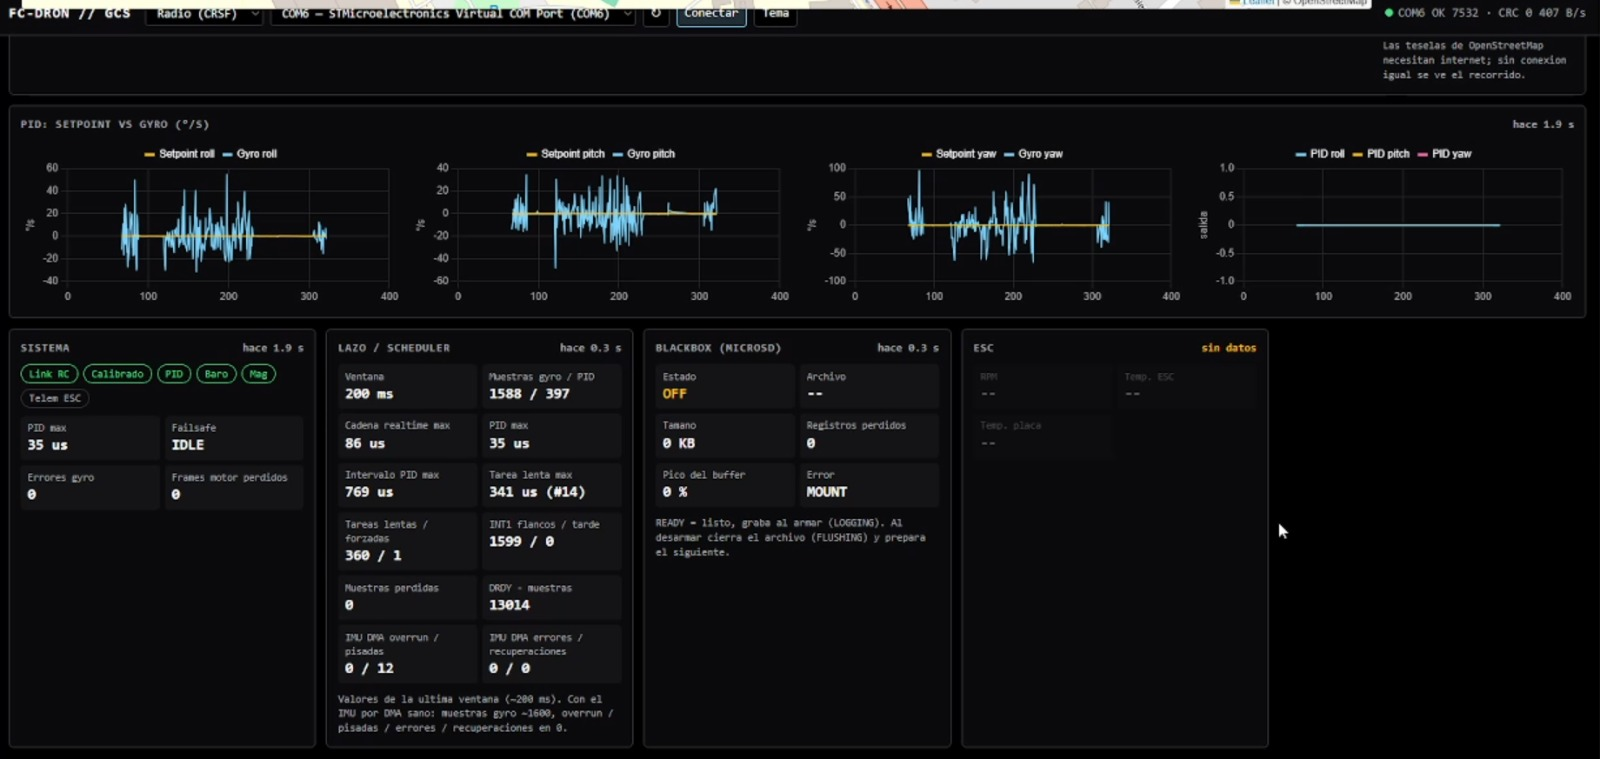
\includegraphics[width=1\linewidth]{GCS_sistema.png}
    \caption{GCS, estado del sistema, lazo de control y scheduler, registro en microSD (blackbox) y ESC.}
    \label{fig:gcs_sistema}
\end{figure}

\subsection{Implementación del GPS}
El controlador integra el módulo GPS HGLRC M100, basado en el receptor u-blox MAX-M10M, conectado al microcontrolador por el puerto \texttt{USART3} (PB10 = TX, PB11 = RX) a 115\,200~baud, 8N1. El módulo transmite sentencias NMEA con su configuración de fábrica (1~Hz), por lo que el pin TX del microcontrolador no se utiliza por ahora.

\paragraph{Recepción no bloqueante.} El \texttt{USART3\_RX} no dispone de un stream DMA libre en el STM32F405 (\texttt{DMA1\_Stream1} está ocupado por DShot), por lo que cada byte se recibe por interrupción \texttt{RXNE} y se almacena en un buffer circular de 512~bytes. A 115\,200~baud llegan como máximo $\approx 11{,}5$~kB/s (un byte cada $\approx 87$~\textmu s), de modo que el buffer aguanta $\approx 44$~ms sin ser vaciado. La interrupción tiene prioridad NVIC 6, numéricamente mayor que la del gyro (EXTI2, prioridad 5), de forma que el GPS nunca retrasa la lectura de la IMU. El buffer se vacía en una tarea lenta del planificador (\texttt{gps\_process}) que corre cada 20~ms con prioridad 2; en cada pasada hay como máximo $\approx 230$~bytes por procesar, es decir, el buffer tiene un margen de $\approx 2{,}2\times$ sobre el peor caso.

\paragraph{Parser NMEA.} Se implementó un parser incremental (carácter a carácter, sin \texttt{float} ni \texttt{double}) que acepta cualquier \textit{talker} (GP, GN, GL, \ldots) y exige checksum XOR válido:
\begin{itemize}
    \item \texttt{GGA}: hora UTC, latitud, longitud, calidad de fix, satélites usados, HDOP y altitud MSL.
    \item \texttt{RMC}: estado (A/V), latitud, longitud, velocidad sobre el suelo y rumbo.
\end{itemize}
Las coordenadas se almacenan como enteros en grados$\times 10^{7}$, la velocidad en cm/s y el rumbo en centésimas de grado.

\paragraph{Validación del fix.} Bajo techo el módulo suele reportar ``fix'' con pocos satélites y HDOP alto, y la posición deriva (recorrido fantasma). Por ello una posición solo se considera válida si cumple simultáneamente: calidad de fix $>0$, al menos 8~satélites, HDOP $\le 2{,}5$ y 3~sentencias GGA buenas consecutivas ($\approx 3$~s a 1~Hz). Si no llega una posición válida durante 2~s, el fix se invalida y la velocidad se pone en cero.

\paragraph{Salida hacia la estación de tierra.} El FC reenvía la posición por el enlace de telemetría como un frame CRSF estándar \texttt{0x02} (GPS) a 1~Hz: latitud y longitud (grados$\times 10^{7}$), velocidad (km/h$\times 10$), rumbo (grados$\times 100$), altitud (m $+1000$) y número de satélites. Se envía a 1~Hz porque el MAX-M10M entrega 1~Hz y un envío más rápido solo repetiría el mismo punto. Mientras no hay fix se envía latitud = longitud = 0, pero se mantiene el número de satélites para que la estación de tierra pueda verificar que el GPS está vivo.

\subsection{Interfaz gráfica de la estación de tierra (GCS)}
Se desarrolló una estación de tierra web (Figuras~\ref{fig:gcs_general} a~\ref{fig:gcs_sistema}) que muestra al dron \textbf{en vuelo}, a través del propio enlace de radio. La cadena de datos es:
\begin{center}
\small
FC (\texttt{fc\_telem.c}) $\xrightarrow{\text{UART4 CRSF}}$ RX ELRS $\xrightarrow{\text{radio 2,4 GHz}}$ TX ELRS $\rightarrow$ EdgeTX $\xrightarrow{\text{USB VCP}}$ \texttt{app.py} $\rightarrow$ navegador
\end{center}
La radio (Radiomaster Pocket) se configura en EdgeTX con \textit{USB-VCP = Telem Mirror}, de modo que reenvía por USB todos los frames CRSF que recibe del dron. Un servidor en Python (Flask) abre ese puerto serie, decodifica los frames con verificación de CRC8 (\texttt{crsf\_link.py}), mantiene el último valor de cada magnitud, la tasa real de cada tipo de frame y series cortas para los gráficos, y los publica al navegador mediante \textit{Server-Sent Events} cada 100~ms. También incluye una fuente simulada (\texttt{--source sim}) que genera frames con el mismo formato byte a byte que el firmware, útil para probar la GUI sin hardware. La interfaz presenta las siguientes tarjetas:
\begin{itemize}
    \item \textbf{Actitud}: horizonte artificial con roll, pitch y yaw (frame 0x1E).
    \item \textbf{Radio / RC}: posición de los sticks, throttle y edad del último frame RC.
    \item \textbf{Motores (DShot)}: valor de los cuatro motores en barras y gráfico temporal.
    \item \textbf{Enlace ELRS}: LQ y RSSI de subida y de bajada, SNR, modo RF y potencia, y una tabla con la tasa real (Hz) de cada tipo de frame frente a la tasa que envía el firmware, con su antigüedad. Esta tabla permite verificar cuánto de lo enviado llega realmente.
    \item \textbf{Batería, Altura / Vario y ESC}: tensión, corriente, consumo, altura relativa, velocidad vertical, RPM y temperaturas.
    \item \textbf{GPS / Mapa}: mapa Leaflet con teselas de OpenStreetMap, recorrido (hasta 1800 puntos, $\approx 30$~min a 1~Hz), punto \textit{home} fijado en el primer fix, distancia a \textit{home}, satélites, velocidad, altitud, rumbo y coordenadas. La flecha del dron sigue el yaw de la brújula mientras el magnetómetro esté en uso y sano; en caso contrario usa el rumbo GPS, atenuado por debajo de 1,5~m/s. Sin conexión a internet se sigue viendo el recorrido, aunque no el mapa base.
    \item \textbf{PID}: setpoint contra gyro filtrado de roll, pitch y yaw, y salida del PID.
    \item \textbf{Sistema, Lazo / scheduler y Blackbox}: banderas de estado (armado, failsafe, calibración, sensores), tiempos máximos del lazo, muestras perdidas, errores del DMA de la IMU y estado del registro en microSD.
\end{itemize}

\subsection{Enlace de telemetría: paquetes, tasas y margen}
\subsubsection{Enlace de subida y de bajada}
El enlace entre el controlador de vuelo y el receptor ELRS es un UART (UART4, PA0/PA1) a 420\,000~baud, 8N1, es decir 10~bits por byte y una capacidad de $42\,000$~B/s en \textbf{cada sentido} (los pines TX y RX son independientes). Todos los frames usan el formato CRSF: \texttt{[sync][len][type][payload][CRC8]}, de modo que el tamaño total de un frame estándar es \textit{payload}\,$+4$~bytes y el de un frame extendido (tipos $\ge$ 0x28, con destino y origen) es \textit{payload}\,$+6$~bytes; el máximo de CRSF es 64~bytes por frame.
\begin{itemize}
    \item \textbf{Subida} (radio $\rightarrow$ dron): un único tipo de frame, \texttt{0x16} \textit{RC Channels Packed}: 16~canales de 11~bits $= 176$~bits $= 22$~bytes de payload, 26~bytes por frame. Se recibe por DMA circular y su tasa es la \textit{packet rate} de ELRS. El firmware considera perdido el enlace si pasan 500~ms sin un frame RC válido, tras lo cual actúa el failsafe.
    \item \textbf{Bajada} (dron $\rightarrow$ radio): varios tipos de frame, cada uno con su propia tasa (Tabla~\ref{tab:frames_bajada}). Se encolan en un buffer de 256~bytes que se transmite por DMA, sin bloquear el lazo de control. Además, ELRS agrega por sí mismo el frame \texttt{0x14} (\textit{Link Statistics}, 10~bytes de payload), que contiene LQ, RSSI y SNR de subida y bajada; no lo genera el firmware.
\end{itemize}

\subsubsection{Paquetes de bajada, tamaño y tasa}
Los datos \textbf{sí se separan en distintos paquetes}: cada magnitud viaja en su propio tipo de frame y con su propia tasa, de acuerdo con qué tan rápido cambia. La actitud, que es lo más dinámico, va a 20~Hz; el GPS, que solo se actualiza a 1~Hz, va a 1~Hz. Los datos de depuración propios del proyecto usan un frame extendido \texttt{0x7F} que alterna dos páginas, cada una a 5~Hz (10~Hz en total).

\begin{table}[htbp]
\centering
\caption{Frames de bajada (FC $\rightarrow$ radio): contenido, tamaño y tasa}
\label{tab:frames_bajada}
\renewcommand{\arraystretch}{1.25}
\footnotesize
\begin{tabular}{@{}l c c c c r p{4.4cm}@{}}
\toprule
\rowcolor{gray!20}
\textbf{Frame} & \textbf{Tipo} & \textbf{Payload} & \textbf{Total} & \textbf{Tasa} & \textbf{Caudal} & \textbf{Contenido} \\
 & & [B] & [B] & [Hz] & [B/s] & \\
\midrule
Attitude & 0x1E & 6 & 10 & 20 & 200 & pitch, roll, yaw (3$\times$int16, rad$\times10^4$) \\
Baro altitude & 0x09 & 2 & 6 & 5 & 30 & altitud barométrica (uint16) \\
Vario & 0x07 & 2 & 6 & 5 & 30 & velocidad vertical (int16, cm/s) \\
Battery & 0x08 & 8 & 12 & 2 & 24 & tensión, corriente, mAh (uint24), \% restante \\
Flight mode & 0x21 & 5--6 & 9--10 & 2 & 20 & texto: ANGL, PASS, CAL*, !FS! ($*$ = desarmado) \\
RPM & 0x0C & 4 & 8 & 2 & 16 & RPM del ESC (int24) \\
Temperature & 0x0D & 5 & 9 & 2 & 18 & temperatura del ESC y de la placa \\
GPS & 0x02 & 15 & 19 & 1 & 19 & lat, lon (int32), velocidad, rumbo, altitud (uint16), satélites (uint8) \\
Debug, pág.~0 & 0x7F & 47 & 53 & 5 & 265 & estado de vuelo (ver abajo) \\
Debug, pág.~1 & 0x7F & 46 & 52 & 5 & 260 & lazo, IMU y blackbox (ver abajo) \\
\midrule
\textbf{Total} & & & & \textbf{49} & \textbf{882} & \\
\textbf{Sin debug} & & & & \textbf{39} & \textbf{357} & \\
\bottomrule
\end{tabular}
\end{table}

\paragraph{Frame de depuración \texttt{0x7F}.} Es un frame propio del proyecto (formato versión 2, big-endian) que se envía como extendido para que ELRS lo reenvíe aunque no conozca el tipo. Alterna dos páginas de 5~Hz cada una:
\begin{itemize}
    \item \textbf{Página 0 (47~B), estado de vuelo:} versión y número de página (2~B); banderas (1~B: armado, failsafe, link RC, calibrado, PID activo, baro, magnetómetro en uso, telemetría ESC válida); flags de bloqueo de armado (1~B); estado de failsafe (1~B); sticks roll/pitch/yaw (3$\times$int16) y throttle (uint16); setpoint de velocidad angular (3$\times$int16); gyro filtrado (3$\times$int16); salida del PID (3$\times$int16); los 4 motores en DShot (4$\times$uint16); tiempo máximo del PID, edad del último frame RC, errores de gyro y frames de motor perdidos (4$\times$uint16).
    \item \textbf{Página 1 (46~B), lazo, IMU y blackbox:} versión y página (2~B); duración de la ventana ($\approx 200$~ms), muestras de gyro y ejecuciones del PID; tiempos máximos de la cadena \textit{realtime}, del PID, del intervalo entre PIDs y de las tareas lentas; contadores de tareas lentas ejecutadas y forzadas; flancos y retrasos de la interrupción DRDY de la IMU y muestras perdidas; \textit{overruns}, muestras pisadas, errores SPI/DMA y recuperaciones del stream de la IMU; y el estado del blackbox (estado, error, archivo, KB escritos, registros perdidos y ocupación máxima del buffer, 1~B).
\end{itemize}
Si cambia este formato, se incrementa el byte de versión y se actualiza el decodificador de la GCS.

\subsubsection{Margen dentro del protocolo}
\paragraph{Margen en el UART FC--receptor.} La suma de todos los frames de bajada es de 882~B/s, el 2,1\,\% de la capacidad de 42\,000~B/s del UART; sin el frame de depuración son 357~B/s (0,85\,\%). El frame más largo (53~B) ocupa 1,26~ms en el cable y deja 11~B de margen respecto del límite de 64~B de CRSF. Aun si todos los frames coincidieran en el mismo instante (133~B), el buffer de transmisión de 256~B quedaría al 52\,\%. En la subida, los frames RC de 26~B a 250~Hz ocupan 6\,500~B/s (15,5\,\% del UART) y a 500~Hz 13\,000~B/s (31\,\%). El UART no es el cuello de botella.

\paragraph{Margen en el enlace de radio.} El verdadero límite es el enlace ELRS. En el aire, todos los paquetes de subida se dedican a los canales RC a la \textit{packet rate} configurada y la telemetría de bajada solo dispone de 1 de cada $N$ paquetes (\textit{Telem Ratio} 1:$N$). Estos parámetros no están definidos en el firmware del FC ni en Betaflight (el código de Betaflight solo conoce el UART CRSF, no la \textit{packet rate} ni el \textit{Telem Ratio}): se configuran en el módulo TX y en el receptor ExpressLRS, por lo que se tomaron del código fuente de ExpressLRS. Allí, los paquetes de 2,4~GHz son de tipo OTA4 (8~bytes, de los cuales 5 son datos útiles; la mayoría de los modos, incluidos 1000, 500, 250 y 150~Hz) u OTA8 (13~bytes, 10 de datos; modos \textit{8CH}). La capacidad de telemetría con paquetes OTA4 es entonces $\text{capacidad} \approx 5\cdot R/N$~B/s, con $R$ la \textit{packet rate} y 1:$N$ el \textit{Telem Ratio} (el máximo permitido es 1:2). La relación por defecto (\textit{Std}) es muy baja: 1:128 a 1000 y 500~Hz, 1:64 a 250~Hz y 1:32 a 150~Hz. La Tabla~\ref{tab:margen_radio} compara estas capacidades con el caudal que genera el firmware.

\begin{center}
Configuración del Radiomaster Pocket: \textit{Packet Rate} = \textbf{PENDIENTE DEFINIR}; \textit{Telem Ratio} = \textbf{PENDIENTE DEFINIR}.
\end{center}

\begin{table}[htbp]
\centering
\caption{Capacidad de telemetría de bajada de ELRS (paquetes OTA4, 5~B por paquete) en B/s según packet rate y Telem Ratio}
\label{tab:margen_radio}
\renewcommand{\arraystretch}{1.25}
\small
\begin{tabular}{@{}c r r r r@{}}
\toprule
\rowcolor{gray!20}
\textbf{Packet rate [Hz]} & \textbf{1:2} & \textbf{1:4} & \textbf{1:8} & \textbf{Std (por defecto)} \\
\midrule
1000 & 2\,500 & 1\,250 & 625 & 39 (1:128) \\
500 & 1\,250 & 625 & 312 & 20 (1:128) \\
250 & 625 & 312 & 156 & 20 (1:64) \\
150 & 375 & 187 & 94 & 23 (1:32) \\
\bottomrule
\end{tabular}
\end{table}

Para transmitir todos los frames a la tasa del firmware (882~B/s) hacen falta al menos $882/5 \approx 177$ paquetes de bajada por segundo; sin el frame de depuración (357~B/s) bastan $\approx 72$. Con el \textit{Telem Ratio} máximo (1:2) los márgenes son:
\begin{itemize}
    \item 1000~Hz: $2\,500-882 = +1\,618$~B/s (65\,\%) con todo el telemetría.
    \item 500~Hz: $1\,250-882 = +368$~B/s (29\,\%) con todo; $+893$~B/s (71\,\%) sin debug. A 1:4 (625~B/s) solo cabe sin debug ($+268$~B/s, 43\,\%).
    \item 250~Hz: $625-357 = +268$~B/s (43\,\%) solo sin debug; con debug no alcanza (71\,\% de lo enviado).
    \item 150~Hz: $375-357 = +18$~B/s (5\,\%) solo sin debug, prácticamente sin margen.
\end{itemize}
Con la relación por defecto (\textit{Std}) la capacidad es de apenas 20 a 40~B/s, muy por debajo de lo que envía el firmware, por lo que es necesario subir el \textit{Telem Ratio} en el módulo TX. Cuando la capacidad no alcanza, ELRS conserva solo el último frame de cada tipo y los rota en sus \textit{slots}, de modo que la tasa recibida cae por debajo de la enviada, sin afectar el control de vuelo, que no depende de la telemetría. El GPS cuesta solo 19~B/s (2,2\,\% del total).

Como referencia, Betaflight limita cada frame de sensor a un máximo de una vez por ciclo de 100~ms (10~Hz; constante \texttt{CRSF\_CYCLETIME\_US}). Con los mismos tamaños de frame, enviar actitud, altitud, batería, modo de vuelo, GPS y vario a 10~Hz equivale a unos 640~B/s (cota superior estimada), más que los 357~B/s del firmware sin debug, que ajusta la tasa de cada magnitud a su dinámica (actitud 20~Hz, GPS 1~Hz).

\paragraph{Tasas medidas en la GCS.} La tarjeta \textit{Enlace ELRS} de la GCS (Figura~\ref{fig:gcs_general}) mide la tasa real con que llega cada tipo de frame a la radio. En la captura con el dron desarmado, los frames llegaron a una fracción de la tasa enviada (Tabla~\ref{tab:tasas_medidas}). El enlace recibía 417~B/s en total, de los cuales unos 59~B/s corresponden a los frames de estadísticas de enlace (4,2~Hz $\times$ 14~B) que genera el propio ELRS, por lo que desde el FC llegan unos 360~B/s, aproximadamente el 41\,\% de los 882~B/s enviados. Los frames de RPM y temperatura no llegaron a la GCS en esa captura. Que el caudal recibido se mantenga alrededor de 360~B/s es consistente con la capacidad de las filas de 312 a 375~B/s de la Tabla~\ref{tab:margen_radio} y confirma que el enlace de radio, y no el UART, es el límite; la fila exacta depende de la configuración del Radiomaster Pocket.

\begin{table}[htbp]
\centering
\caption{Tasa de cada frame: enviada por el firmware y recibida en la GCS}
\label{tab:tasas_medidas}
\renewcommand{\arraystretch}{1.25}
\small
\begin{tabular}{@{}l r r@{}}
\toprule
\rowcolor{gray!20}
\textbf{Frame} & \textbf{Enviada [Hz]} & \textbf{Recibida [Hz]} \\
\midrule
Attitude & 20 & 2,6 \\
Baro altitude & 5 & 2,6 \\
Vario & 5 & 2,6 \\
Battery & 2 & 2,2 \\
Flight mode & 2 & 1,7 \\
GPS & 1 & 1,1 \\
Debug, pág.~0 y 1 (total) & 10 & 4,8 \\
Link statistics (ELRS) & -- & 4,2 \\
\bottomrule
\end{tabular}
\end{table}

\paragraph{Margen en el enlace de subida.} Cada paquete de subida lleva canales RC, por lo que el margen no se mide en ancho de banda sino en tolerancia a pérdidas: el failsafe se activa a los 500~ms sin frames RC válidos, es decir, tras $\approx 125$ frames consecutivos perdidos a 250~Hz (un frame cada 4~ms) o $\approx 250$ a 500~Hz. El indicador de LQ de subida y de bajada del GCS permite vigilar este margen en tiempo real.

\paragraph{Nota.} Los 5~bytes por paquete de bajada se obtienen del formato OTA4 de ExpressLRS (8~bytes menos 3 de cabecera y CRC); no se verificó en el código de ExpressLRS cómo se fragmentan los frames CRSF en esos paquetes, por lo que la capacidad es una estimación teórica. En este proyecto el emisor es el Radiomaster Pocket, cuyo módulo ELRS 2,4~GHz es interno; la \textit{packet rate} y el \textit{Telem Ratio} se leen y se cambian desde el script Lua de ELRS en EdgeTX (opciones \textit{Packet Rate} y \textit{Telem Ratio}) y deben confirmarse allí, ya que de ellos depende la fila aplicable de la Tabla~\ref{tab:margen_radio}. Además, la tasa efectivamente recibida se puede verificar con la tabla de ``Frame rates'' de la tarjeta \textit{Enlace ELRS} del GCS.

% 8. Costos
\section{Componentes}
\subsection{Selección de los motores}

La elección del motor se tomó atendiendo a dos criterios críticos: el consumo 
de corriente y el empuje (\textit{thrust}). El consumo determina el tiempo de 
vuelo disponible, por lo que resulta conveniente seleccionar motores con una 
constante $K_v$ inferior a la habitual manteniendo un diámetro de rotor 
reducido; el empuje, por su parte, condiciona la velocidad máxima, la rapidez 
de respuesta del vehículo y su capacidad de carga.

Dado que el alcance del proyecto persigue un diseño equilibrado entre autonomía 
y agilidad, y no un vehículo especializado en \textit{long range} ni en 
\textit{freestyle} agresivo, se acotó la búsqueda al rango de 
\SIrange{1500}{1750}{\kilo\volt}. Este intervalo ofrece un compromiso adecuado 
entre el par disponible para hélices de \SI{6}{in} y un consumo contenido en 
régimen de crucero. Finalmente se seleccionó un motor \textit{brushless} Xing 
2306 de \SI{1700}{\kilo\volt}, decisión condicionada por criterios de 
disponibilidad comercial y presupuesto.

\subsection{Selección de las hélices}

Con el fin de maximizar el empuje se optaron por hélices tripala. Esta 
configuración presenta como contrapartida una mayor generación de turbulencia y 
una menor eficiencia energética frente a las bipala, si bien dicho efecto 
resulta determinante únicamente en aplicaciones cinematográficas, donde la 
estabilidad de la imagen es prioritaria. Al no ser este el caso del proyecto, se 
consideró aceptable la penalización.

Se seleccionaron hélices \textbf{6030}, cuya denominación indica un diámetro de 
\SI{6}{in} (\SI{0.1524}{\meter}) y un paso (\textit{pitch}) de \SI{3.0}{in} 
(\SI{0.0762}{\meter}).

\subsection{Cálculo del empuje}

El empuje generado por cada hélice se obtiene a partir de la ecuación~\eqref{eq:thrust}:

\begin{equation}
T = C_T \, \rho \, n^{2} D^{4}
\label{eq:thrust}
\end{equation}

\noindent donde:

\begin{description}
  \item[$T$ (\textit{Thrust}).] Empuje total generado, expresado en newtons en 
  el Sistema Internacional, aunque en el ámbito del \textit{hobby} suele 
  indicarse en gramos-fuerza.
  \item[$C_T$ (coeficiente de empuje).] Valor adimensional que depende de la 
  geometría de la hélice, del ángulo de ataque (\textit{pitch}) y, de forma 
  determinante, del número de palas. Para una hélice 6030 tripala su valor 
  estimado se sitúa entre 0.10 y 0.12.
  \item[$\rho$ (densidad del aire).] A nivel del mar toma el valor aproximado 
  de \SI{1.225}{\kilo\gram\per\meter\cubed}.
  \item[$n$.] Velocidad de rotación expresada en revoluciones por segundo (RPS).
  \item[$D$.] Diámetro de la hélice en metros; para \SI{6}{in}, 
  $D = \SI{0.1524}{\meter}$.
\end{description}

\subsubsection{Cálculo de la velocidad de rotación}

La velocidad de giro teórica en vacío se obtiene mediante la 
ecuación~\eqref{eq:rpm}:

\begin{equation}
\text{RPM}_{\text{máx}} = K_v \cdot V
\label{eq:rpm}
\end{equation}

Para la batería 6S plenamente cargada (\SI{25.2}{\volt}):

\begin{equation}
\text{RPM}_{\text{máx}} = 1700 \times 25.2 = \SI{42840}{rpm}
\end{equation}

No obstante, la configuración tripala incrementa la resistencia aerodinámica y 
el motor no alcanza su velocidad en vacío. En condiciones reales de vuelo, con 
el acelerador al \SI{100}{\percent}, los motores giran aproximadamente entre el 
\SIrange{80}{85}{\percent} de las RPM teóricas máximas debido a esta carga de 
trabajo. Se adopta por tanto:

\begin{equation}
n = \SI{36000}{rpm} = \SI{600}{rps}
\end{equation}

\subsubsection{Resultado}

Sustituyendo en la ecuación~\eqref{eq:thrust} con $C_T = 0.12$:

\begin{align}
T &= 0.12 \times 1.225 \times (600)^{2} \times (0.1524)^{4} \\
T &\approx \SI{28.55}{\newton}
\end{align}

Expresado en gramos-fuerza:

\begin{equation}
\text{Empuje}_{\text{unitario}} = \frac{28.55}{9.81} \times 1000 \approx \SI{2910}{\gram}
\end{equation}

\begin{equation}
\text{Empuje}_{\text{total}} = 2910 \times 4 = \SI{11640}{\gram}
\end{equation}

\paragraph{Observación sobre el coeficiente de empuje.}
El coeficiente $C_T$ constituye una aproximación que debe determinarse 
experimentalmente, dado que cada modelo de hélice presenta un comportamiento 
distinto. Para este trabajo se partió de un valor tabulado obtenido a partir de 
las mediciones de la base de datos \textit{UIUC Propeller Data Site}, 
Vols.~1--2 \cite{ref7}. La expresión que permite despejarlo a partir de 
medidas experimentales es la ecuación~\eqref{eq:ct}:

\begin{equation}
C_T = \frac{T}{\rho \, n^{2} D^{4}}
\label{eq:ct}
\end{equation}

\noindent donde $T$ se obtiene mediante ensayo en banco de empuje y $n$ se mide 
simultáneamente con un tacómetro óptico o a partir de la telemetría del ESC.

\subsection{Modelado del motor y empuje real}

El valor de la ecuación~\eqref{eq:thrust} depende de $C_T$ y de las RPM supuestas, por lo que se lo contrastó con una identificación experimental del conjunto ESC + motor + hélice (Xing 2306 1700~kV con hélice 6030 tripala, alimentación 6S), la misma que se utilizó para el modelo del motor del balancín de dos motores con control PID.

\paragraph{Ensayo.} En un banco de empuje se aplicaron escalones de throttle (comando DShot) de 30\,\% y de 50\,\% y se registró el empuje con un período de muestreo de 2,5~ms (Figura~\ref{fig:empuje_motor}, izquierda). Con la \textit{System Identification Toolbox} de MATLAB (\texttt{tfest}) se ajustaron modelos de primer y segundo orden, con el throttle (en \%) como entrada y el empuje como salida (en N, según la unidad de la celda de carga del banco, supuesta en newtons).

\begin{figure}[htbp]
    \centering
    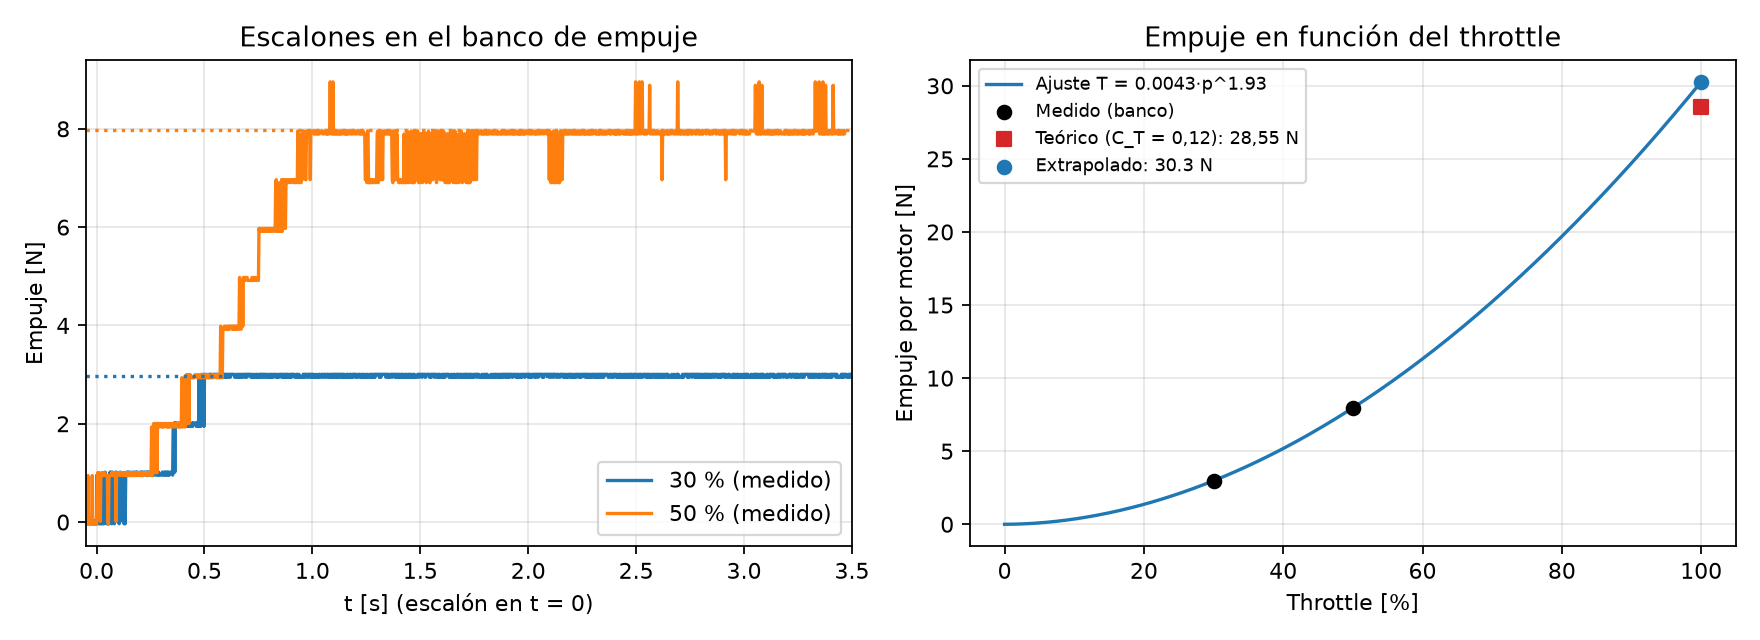
\includegraphics[width=\linewidth]{Empuje_motor.png}
    \caption{Izquierda: escalones de throttle de 30\,\% y 50\,\% medidos en el banco. Derecha: empuje por motor en función del throttle, ajuste a los dos puntos medidos y comparación con el valor teórico al 100\,\%.}
    \label{fig:empuje_motor}
\end{figure}

\begin{table}[htbp]
\centering
\caption{Modelos identificados del motor ($G(s)$ en N/\%)}
\label{tab:modelo_motor}
\renewcommand{\arraystretch}{1.3}
\small
\begin{tabular}{@{}c c c c c@{}}
\toprule
\rowcolor{gray!20}
\textbf{Escalón} & \textbf{Empuje en régimen} & \textbf{Ganancia estática} & \textbf{$G(s)$, 2 polos} & \textbf{Ajuste} \\
\midrule
30\,\% & 2.98~N & 0.099~N/\% & $\dfrac{2.337}{s^{2}+6.807\,s+23.65}$ & 76.6\,\% \\
50\,\% & 7.97~N & 0.157~N/\% & $\dfrac{1.535}{s^{2}+4.941\,s+9.804}$ & 81.0\,\% \\
\bottomrule
\end{tabular}
\end{table}

La ganancia estática no es constante: pasa de 0.099~N/\% a 30\,\% a 0.157~N/\% a 50\,\%, es decir, el empuje no es lineal con el throttle, como cabe esperar de $T \propto n^{2}$. Por ello, un único valor de ganancia solo describe el comportamiento cerca de un punto de operación. Para estimar el empuje máximo se ajustó una ley de potencia $T = a\,p^{\,b}$ ($p$ en \%) a los dos regímenes medidos:
\begin{align*}
b &= \frac{\ln(7.97/2.98)}{\ln(50/30)} = 1.93, \\
a &= \frac{7.97}{50^{1.93}} = 4.26\times10^{-3}\ \text{N}, \\
T(100\,\text{\%}) &= 4.26\times10^{-3}\cdot 100^{1.93} \approx 30.3\ \text{N}
\end{align*}
El exponente cercano a 2 es consistente con la ecuación~\eqref{eq:thrust}. Con otro criterio de ajuste (raíz cuadrada del empuje lineal con el throttle) el resultado es 31.0~N, es decir, el valor extrapolado es robusto al modelo elegido, dentro de $\approx 2\,\text{\%}$.

\paragraph{Comparación con el valor teórico.} La Tabla~\ref{tab:comparacion_empuje} compara ambos resultados y calcula cuánta carga podría levantar el dron, tomando una masa del dron de \SI{900}{\gram} (sección anterior) y $g = 9.81~\text{m/s}^2$. El margen del 2:1 corresponde a la relación empuje/peso mínima habitual para mantener control en vuelo, es decir, que el dron levante la carga con el 50\,\% del empuje máximo.

\begin{table}[htbp]
\centering
\caption{Empuje teórico frente a empuje real extrapolado (100\,\% de throttle, 4 motores)}
\label{tab:comparacion_empuje}
\renewcommand{\arraystretch}{1.3}
\small
\begin{tabular}{@{}l r r r@{}}
\toprule
\rowcolor{gray!20}
\textbf{Magnitud} & \textbf{Teórico} & \textbf{Real (modelo)} & \textbf{Diferencia} \\
\midrule
Empuje por motor [N] & 28.55 & 30.3 & $+6.0\,\text{\%}$ \\
Empuje por motor [gf] & 2910 & 3086 & $+6.0\,\text{\%}$ \\
Empuje total, 4 motores [kgf] & 11.64 & 12.34 & $+6.0\,\text{\%}$ \\
$C_T$ equivalente (a 600~rps) & 0.120 & 0.127 & \\
Relación empuje/peso (dron de 0.9~kg) & 12.9 & 13.7 & \\
Carga máxima a 100\,\% de empuje [kg] & 10.7 & 11.4 & \\
Carga con margen 2:1 (50\,\% del empuje) [kg] & 4.9 & 5.3 & \\
\bottomrule
\end{tabular}
\end{table}

Con el modelo real, los cuatro motores generan unos \textbf{12.3~kgf} de empuje total, de modo que el dron (0.9~kg) podría elevar una carga adicional de hasta $\approx 11.4$~kg a máxima potencia y de $\approx 5.3$~kg conservando un margen 2:1 (el valor teórico predice 10.7~kg y 4.9~kg, respectivamente). Para sostener el dron en vuelo estacionario sin carga se necesitan $0.9 \times 9.81/4 = 2.21$~N por motor, que según el modelo corresponde a un throttle de $\approx 26\,\text{\%}$.

\paragraph{Limitaciones.}
\begin{itemize}
    \item El banco solo se ensayó hasta 50\,\% de throttle: el empuje al 100\,\% es una extrapolación a partir de dos puntos y no una medición directa.
    \item La caída de tensión de la batería y la limitación de corriente del ESC a plena potencia pueden reducir el empuje real por debajo del extrapolado.
    \item La unidad de la celda de carga del banco se supone en newtons; la coincidencia con el valor teórico (diferencia del 6\,\%) respalda esta suposición.
    \item El $C_T$ equivalente supone las 36\,000~rpm adoptadas en el cálculo teórico, no medidas; si las RPM reales fueran distintas cambiaría el $C_T$ pero no el empuje.
\end{itemize}

\subsection{Selección de la batería}

Para la alimentación del sistema se optó por una configuración 6S, opción 
intermedia entre los vehículos orientados a \textit{long range} y los de 
\textit{freestyle}. Al operar con una tensión más elevada, el sistema demanda 
menor corriente para una misma potencia entregada, lo que reduce las pérdidas 
óhmicas en el cableado y en los variadores, y permite una mayor autonomía de 
vuelo.

La elección de una tasa de descarga de 120C responde a que los motores 
seleccionados pueden alcanzar picos del orden de \SI{40}{\ampere} cada uno. 
Para la batería LiPo escogida, de \SI{1300}{\milli\ampere\hour}, la corriente 
de pico disponible resulta:

\begin{equation}
I_{\text{pico}} = 1.3 \times 120 = \SI{156}{\ampere}
\end{equation}

\subsection{Consumo y autonomía estimada}

En régimen de crucero, un \textit{frame} de \SI{6}{in} con una masa aproximada 
de \SI{900}{\gram} equipado con los motores Xing E-Pro 2306 de 
\SI{1700}{\kilo\volt} presenta un consumo global comprendido entre 
\SIrange{20}{30}{\ampere}. La autonomía estimada con una batería de 
\SI{1300}{\milli\ampere\hour} se resume en la Tabla~\ref{tab:autonomia}.

\begin{table}[htbp]
\centering
\caption{Autonomía estimada según el perfil de vuelo.}
\label{tab:autonomia}
\begin{tabular}{@{}ll@{}}
\toprule
\textbf{Perfil de vuelo} & \textbf{Autonomía estimada} \\
\midrule
Vuelo eficiente / \textit{long range} & \SIrange{5}{7}{\minute} \\
Vuelo mixto (crucero y maniobras)     & \SIrange{4}{5}{\minute} \\
Vuelo agresivo                        & \SIrange{3}{4}{\minute} \\
\bottomrule
\end{tabular}
\end{table}
\pagebreak

\subsection{Materiales y herramientas compradas/incremental}

\begin{table}[htbp]
\centering
\caption{Materiales adquiridos para el prototipo}
\label{tab:materiales_comprados}
\renewcommand{\arraystretch}{1.3}
\setlength{\tabcolsep}{8pt}
\begin{tabularx}{\textwidth}{@{}Xccc@{}}
\toprule
\rowcolor{gray!20}
\textbf{Objeto} & \textbf{Cantidad} & \textbf{Precio (USD)} & \textbf{Subtotal (USD)} \\
\midrule
RadioMaster Pocket CC2500 & 1 & 59.99 & 59.99 \\
ELRS 2.4TX module AION 2.4TX NANO & 1 & 29.99 & 29.99 \\
BetaFPV SuperD RX ELRS 2.4\,GHz & 1 & 19.99 & 19.99 \\
XING EPro 2306 1700KV & 4 & 16.99 & 67.96 \\
ChinaHobbyLine 1300mAh 120C 6S & 1 & 17.99 & 17.99 \\
Hélices 6030 Midnight Gray 2L2R (AliExpress) & 1 & 4.50 & 4.50 \\
\midrule
\textbf{Total} & & & \textbf{200.42} \\
\bottomrule
\end{tabularx}
\end{table}

\subsection{Materiales y herramientas prestadas/existentes}

Los componentes principales de la PCB del controlador de vuelo se adquirieron en LCSC. El costo total del pedido de componentes fue de 60~USD.

\begin{table}[htbp]
\centering
\caption{Componentes de la PCB adquiridos en LCSC}
\label{tab:componentes_pcb}
\renewcommand{\arraystretch}{1.3}
\setlength{\tabcolsep}{8pt}
\begin{tabularx}{\textwidth}{@{}Xccc@{}}
\toprule
\rowcolor{gray!20}
\textbf{Objeto} & \textbf{Cantidad} & \textbf{Precio (USD)} & \textbf{Subtotal (USD)} \\
\midrule
STM32F405RGT6 & 2 & 6.67 & 13.34 \\
IMU LSM6DSV16XTR & 2 & 4.46 & 8.92 \\
Barómetro BMP388 & 2 & 3.94 & 7.88 \\
Magnetómetro MMC5983MA & 2 & 2.27 & 4.54 \\
Otros componentes & 1 & 25.32 & 25.32 \\
\midrule
\textbf{Total} & & & \textbf{60.00} \\
\bottomrule
\end{tabularx}
\end{table}

\section{Resultados parciales y finales}

\subsection{Pruebas realizadas: telemetría de sensores y motores}

Se completó de forma satisfactoria la recepción de telemetría a través de la interfaz USB. En particular, se verificó la lectura del giroscopio, del acelerómetro, del estado de la batería y del consumo de los motores, además de las lecturas del magnetómetro mostradas en la Figura~\ref{fig:pruebas_usb_mag}.

\begin{itemize}
    \item \textbf{Telemetría de sensores inerciales:} se recibieron correctamente las muestras del giroscopio y del acelerómetro, confirmando la comunicación con la IMU y la coherencia de los ejes.

    \item \textbf{Telemetría de batería:} se obtuvo la tensión y el estado de la batería 6S en tiempo real desde el controlador de vuelo.

    \item \textbf{Lectura de consumo de motores:} se recibió la telemetría de corriente de los motores, lo que permite monitorear el consumo durante las pruebas en banco.

    \item \textbf{Interfaz serie de control:} los datos se visualizaron por USB, validando el enlace entre la FC CORVUS y la estación en tierra.
\end{itemize}

\begin{figure}[H]
    \centering
    \begin{subfigure}[b]{0.48\linewidth}
        \centering
        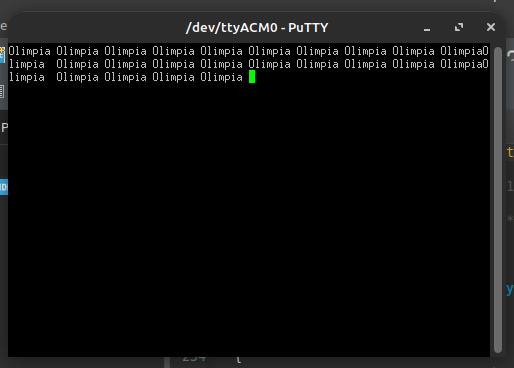
\includegraphics[width=\linewidth]{printOlimpia.png}
        \caption{Lectura serial del USB.}
        \label{fig:usb}
    \end{subfigure}
    \hfill
    \begin{subfigure}[b]{0.48\linewidth}
        \centering
        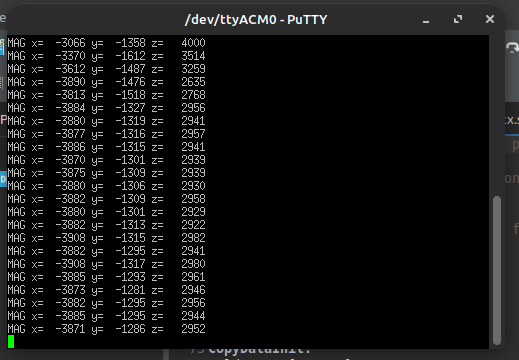
\includegraphics[width=\linewidth]{Magnetometro.png}
        \caption{Lecturas del magnetómetro.}
        \label{fig:magnetometro}
    \end{subfigure}
    \caption{Pruebas de la interfaz USB y del magnetómetro.}
    \label{fig:pruebas_usb_mag}
\end{figure}

\subsection{Prueba del GPS en exteriores}

Se realizó una prueba del GPS a la intemperie, con el controlador de vuelo alimentado y la telemetría enviada por el enlace ELRS hasta la estación de tierra, donde la GCS (Figura~\ref{fig:gps_test}) mostró la posición y el recorrido en tiempo real sobre el mapa. El módulo se llevó caminando fuera del edificio y de vuelta a la zona de partida.

\paragraph{Configuración del GPS durante la prueba.} Los umbrales que definen cuándo una posición se considera válida son los del driver descrito en la implementación del GPS:
\begin{itemize}
    \item \textbf{Satélites mínimos:} 8 (\texttt{GPS\_MIN\_SATS}); con menos satélites la posición se descarta.
    \item \textbf{HDOP máximo:} 2,5 (\texttt{GPS\_MAX\_HDOP\_X100} = 250).
    \item \textbf{Racha de sentencias buenas:} 3 sentencias GGA consecutivas ($\approx 3$~s a 1~Hz) antes de declarar el fix válido (\texttt{GPS\_GOOD\_STREAK}).
    \item \textbf{Vencimiento del fix:} 2~s sin una posición válida (\texttt{GPS\_FIX\_TIMEOUT\_MS}) invalidan el fix y ponen la velocidad en cero.
    \item \textbf{Calidad de fix:} mayor que 0 en la sentencia GGA, con coordenadas válidas y checksum correcto.
    \item \textbf{Enlace:} USART3 a 115\,200~baud, sentencias GGA y RMC a 1~Hz, buffer de recepción de 512~bytes; frame CRSF 0x02 hacia tierra a 1~Hz.
\end{itemize}
Estos umbrales evitan el ``recorrido fantasma'' que se observa cuando el módulo reporta fix con pocos satélites y la posición deriva.

\begin{figure}[H]
    \centering
    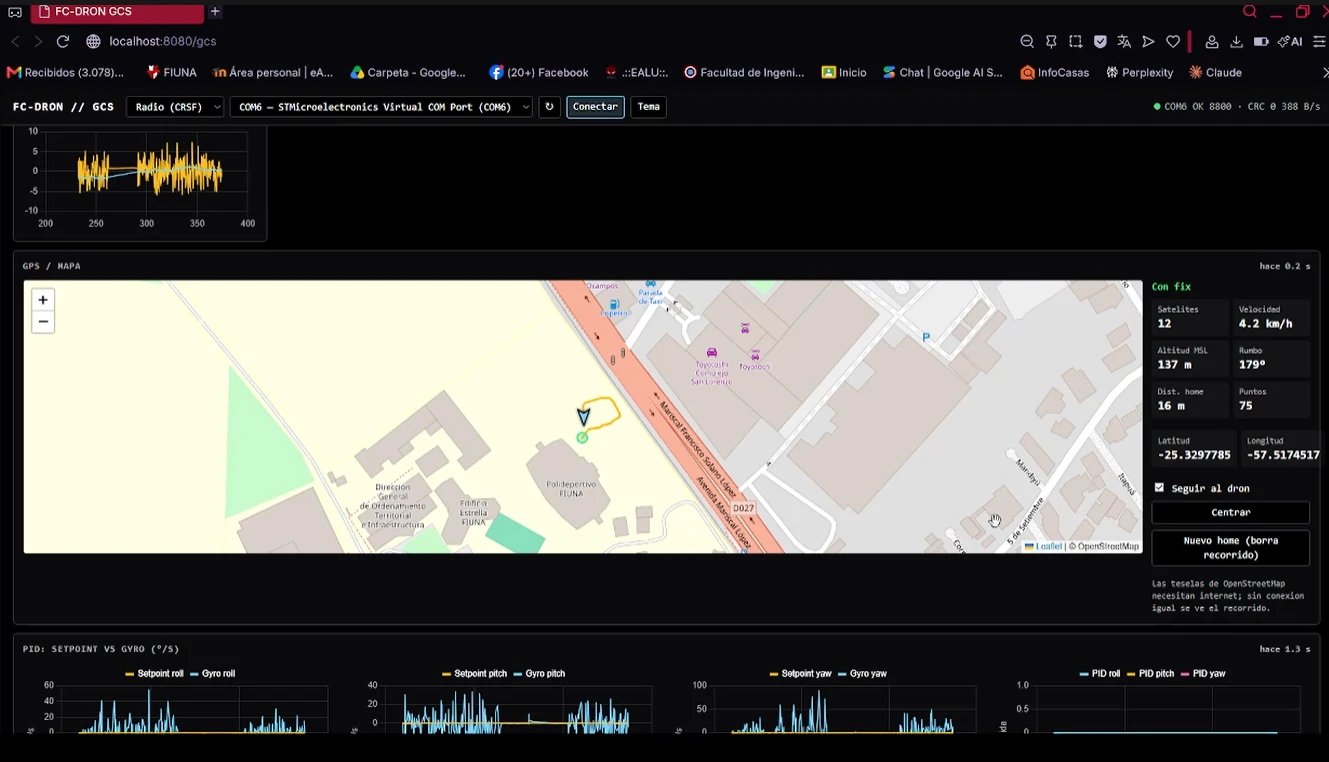
\includegraphics[width=\linewidth]{GCS_GPS_test.png}
    \caption{GCS durante la prueba del GPS en exteriores: mapa con la posición del dron, \textit{home} (círculo verde) y recorrido (línea amarilla).}
    \label{fig:gps_test}
\end{figure}

\paragraph{Resultados.} La prueba fue exitosa:
\begin{itemize}
    \item El GPS obtuvo fix con \textbf{12 satélites}, por encima del mínimo configurado de 8.
    \item La posición y el recorrido se actualizaron en tiempo real en el mapa (75 puntos registrados en la captura, uno por segundo), con la flecha del dron siguiendo el rumbo ($179^\circ$) y una velocidad de 4,2~km/h acorde a la marcha a pie.
    \item Se mostraron correctamente las coordenadas ($-25{,}3297785$, $-57{,}5174517$), la altitud MSL (137~m) y la distancia al punto de partida (\textit{home}): 16~m en la captura.
    \item Al regresar al punto de partida, el error de distancia a \textit{home} fue de entre 1 y 2~m.
    \item El enlace de telemetría funcionó sin errores en la captura: 8\,800 frames válidos, 0 errores de CRC y 388~B/s recibidos.
\end{itemize}

\subsection{Prueba en mástil: reacción del PID}

Para observar la respuesta del lazo de control sin necesidad de volar, el dron se montó sobre un mástil (Figura~\ref{fig:test_mastil}). El mástil es de diseño propio y se fija a una base impresa que lo mantiene estable sobre el suelo. En su extremo superior, el dron se apoya sobre un acople que permite los \textbf{tres grados de libertad} de rotación (alabeo, cabeceo y guiñada); este acople fue adaptado de un soporte de cámara. El apoyo se hace a través del acople para el apoyo de aterrizaje y el mástil descrito en el diseño mecánico, de modo que el dron puede inclinarse y girar libremente sobre el punto de apoyo mientras sus motores se mantienen fuera del contacto con el suelo.

\begin{figure}[H]
    \centering
    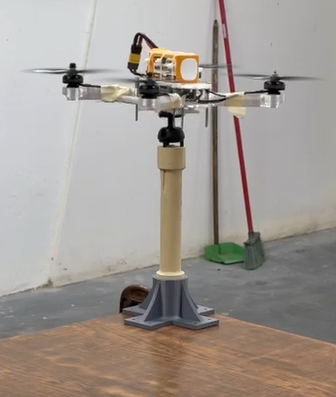
\includegraphics[height=9cm, keepaspectratio]{Test_mastil.png}
    \caption{Prueba en mástil: el dron montado sobre un acople de tres grados de libertad para observar la reacción del PID.}
    \label{fig:test_mastil}
\end{figure}

Con esta disposición, una perturbación de la actitud (por ejemplo, inclinar el dron con la mano) produce una velocidad angular que el giroscopio mide y el controlador debe corregir mediante la diferencia de empuje entre los motores, igual que en vuelo pero sin el riesgo de un despegue. Así se puede verificar el signo de cada eje, la dirección de las correcciones, la respuesta amortiguada del lazo en cascada (ángulo y velocidad angular) y la estabilidad ante perturbaciones, antes de pasar al primer vuelo.

\paragraph{Parámetros del PID.} La prueba se realizó con el controlador en modo \textit{ANGLE}: un lazo externo de ángulo ($K_\theta = 5$~(°/s)/° sobre el error de ángulo, con ángulo máximo de $30^\circ$ y velocidad angular de referencia limitada a 150~°/s) y un lazo interno PID de velocidad angular, ejecutado a 2~kHz con el giroscopio a 8~kHz. Las ganancias están expresadas en las unidades de Betaflight y se escalan por constantes propias de ese firmware, con un factor global de 0,6 (Tabla~\ref{tab:pid_mastil}).

\begin{table}[htbp]
\centering
\caption{Parámetros del PID utilizados en la prueba en mástil}
\label{tab:pid_mastil}
\renewcommand{\arraystretch}{1.3}
\small
\begin{tabular}{@{}l c c c@{}}
\toprule
\rowcolor{gray!20}
\textbf{Eje} & \textbf{P} & \textbf{I} & \textbf{D} \\
\midrule
Roll & 45 & 80 & 40 \\
Pitch & 47 & 84 & 46 \\
Yaw & 45 & 80 & 0 \\
\bottomrule
\end{tabular}
\end{table}

Los valores se multiplican por las constantes de escala de Betaflight ($0{,}032029$ para P, $0{,}244381$ para I y $0{,}000529$ para D), por el factor global 0,6 y, en el caso del D, por un factor adicional de 0,5. Así, las ganancias efectivas del eje de roll son $K_p = 0{,}865$, $K_i = 11{,}7$ y $K_d = 6{,}35\times10^{-3}$. El D se filtra con dos pasa bajos de 75 y 150~Hz, y la suma de los términos se limita a 250 (200 en yaw), con el término integral limitado a 150.

\paragraph{Resultados.} Con estos parámetros el controlador mostró una \textbf{buena velocidad de reacción} ante las perturbaciones de la actitud y parece tener \textbf{buena precisión} al volver a la referencia. Queda pendiente cuantificar estas observaciones (sobreimpulso, tiempo de establecimiento y error en régimen) a partir de los registros de la prueba.

\subsection{Pruebas a realizar}
Restan las pruebas de integración mecánica y de control en vuelo:

\begin{itemize}
    \item \textbf{Rigidez estructural:} verificar la resistencia y la rigidez del chasis True~X bajo carga, de modo que las vibraciones no degraden la estimación de actitud.

    \item \textbf{Sintonización PID:} ajustar los coeficientes del lazo de control para conseguir la estabilización del dron en hover, con respuesta amortiguada ante perturbaciones.

    \item \textbf{Vuelo del dron:} realizar el primer vuelo de validación una vez superadas las pruebas estructurales y de control.
\end{itemize}
\pagebreak
\section{Conclusiones parciales}

Hasta el momento se ha validado satisfactoriamente la cadena de adquisición y 
transmisión de telemetria del controlador de vuelo CORVUS. La recepción por 
interfaz USB permitió verificar la lectura coherente del giroscopio, el 
acelerómetro y el magnetómetro, confirmando la correcta comunicación con la 
unidad inercial y la consistencia en la orientación de los ejes. Asimismo, se 
obtuvieron en tiempo real la tensión y el estado de la batería 6S, junto con la 
telemetria de corriente de los motores, lo que habilita el monitoreo del consumo 
durante los ensayos en banco. Estos resultados validan el enlace serie entre la 
FC CORVUS y la estación en tierra, cumpliendo con los objetivos específicos 
relativos a la selección del protocolo y a la transmisión de telemetría.

Queda pendiente la integración mecánica y la validación del lazo de control en 
vuelo. En las próximas etapas se abordarán la verificación de la rigidez 
estructural del chasis \textit{True X} bajo carga, de modo que las vibraciones 
no degraden la estimación de actitud; la sincronización de los coeficientes PID 
para lograr una estabilización amortiguada en \textit{hover}; y, finalmente, el 
primer vuelo del vehículo, que permitirá contrastar en condiciones reales los 
valores de empuje y autonomía estimados analíticamente.

% 11. Bibliografía
\bibliographystyle{IEEEtran}
\begin{thebibliography}{99}
    \bibitem{ref1} M. Strohmeier, ``FARN - A Novel UAV Flight Controller for Highly Accurate and Reliable Navigation,'' Tesis Doctoral, Julius-Maximilians-Universität Würzburg, Würzburg, Alemania, 2021. [En línea]. Disponible: \url{https://opus.bibliothek.uni-wuerzburg.de/frontdoor/index/index/docId/22313}

    \bibitem{ref2} H. Lyu, ``Multivariable Control of a Rolling Spider Drone,'' Tesis de Maestría, University of Rhode Island, Rhode Island, EE. UU., 2017. [En línea]. Disponible: \url{https://digitalcommons.uri.edu/theses/1130/}

    \bibitem{ref3} N. Van Hien, V.-T. Truong y N.-T. Bui, ``An Object-Oriented Systems Engineering Point of View to Develop Controllers of Quadrotor Unmanned Aerial Vehicles,'' \textit{International Journal of Aerospace Engineering}, vol. 2020, Art. no. 8862864, 2020. [En línea]. Disponible: \url{https://onlinelibrary.wiley.com/doi/epdf/10.1155/2020/8862864}

    \bibitem{ref4} D. Kharolia, J. Singh y M. Kothari, ``Autopilot Design and Development for Multirotor UAVs,'' en \textit{AIAA SCITECH 2024 Forum}, Orlando, FL, EE. UU., Ene. 2024, Art. no. 1698. [En línea]. Disponible: \url{https://arc.aiaa.org/doi/10.2514/6.2024-1698}

    \bibitem{ref5} B. W. McCormick, \textit{Aerodynamics, Aeronautics, and Flight Mechanics}, 2ª ed. New York, NY, EE. UU.: John Wiley \& Sons, 1995.

    \bibitem{ref6} A. Lashmar, ``Calculate Propeller Thrust for Peak Drone Performance,'' \textit{Evolution Flight}, Sep. 2025. [En línea]. Disponible: \url{https://evolutionflight.com/calculate-propeller-thrust/}

    \bibitem{ref7} J. B. Brandt, R. W. Deters y M. S. Selig, \textit{UIUC Propeller Data Site}, Vols. 1--2, Dept. Aerosp. Eng., Univ. Illinois Urbana-Champaign, Urbana, IL, EE. UU., 2012. [En línea]. Disponible: \url{https://m-selig.ae.illinois.edu/props/propDB.html}
\end{thebibliography}


\end{document}